\begin{appendices}

\chapter{Mockups de Interfaces del Sistema}
\label{anexo:Mockups}

% ------------------------------------------------------------------------------
% SECCIÓN 1: PERFIL QUEJOSO
% ------------------------------------------------------------------------------
\section{Perfil: Quejoso}
Este perfil esta relacionado con la comunidad politécnica, toda aquella persona pertenenciete al instituto, al presentar una queja, se convierte directamente en un 'quejoso'.

% --- VISTA 01 ---
\begin{figure}[h]
    \centering
    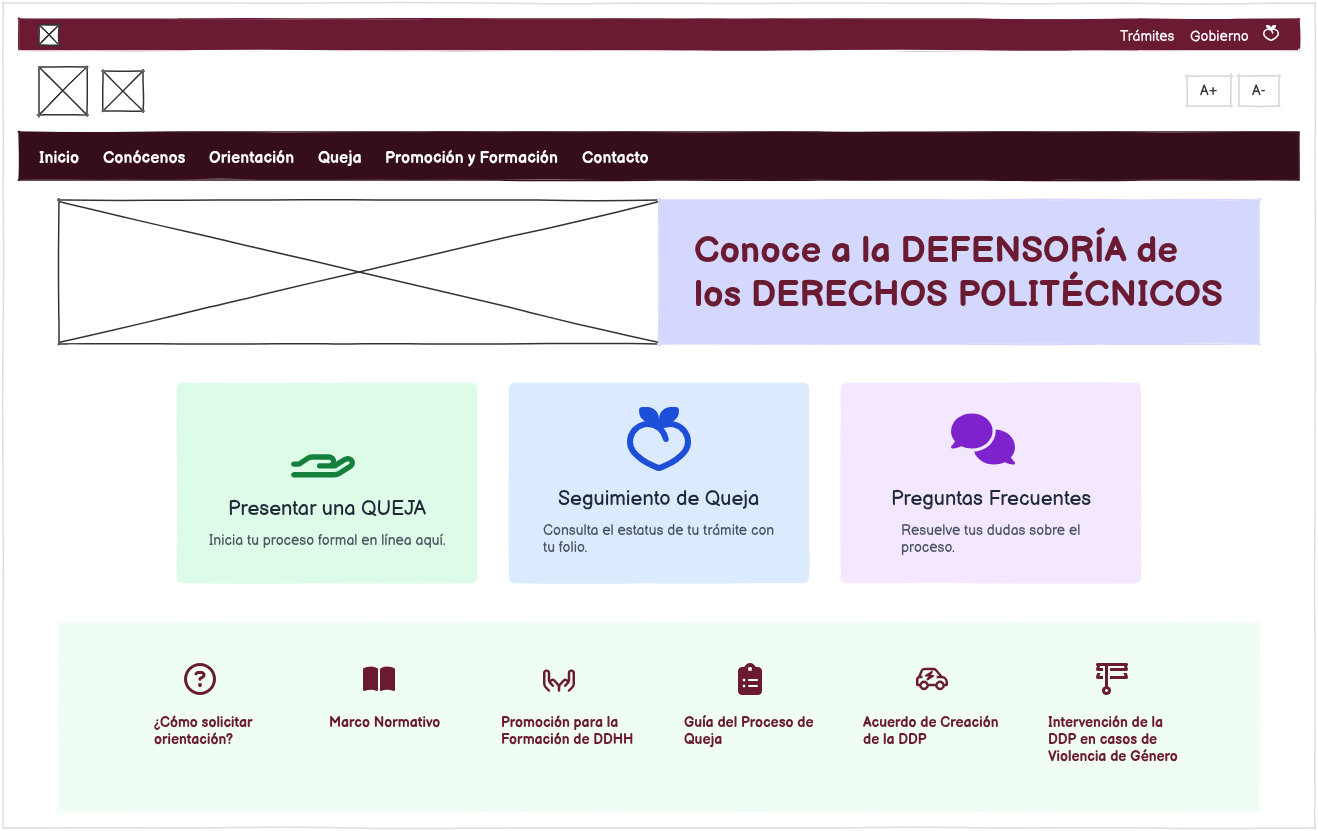
\includegraphics[width=0.65\textwidth]{imagenes/quejoso/Inicio.png}
    \caption{MQ-01: Pantalla de inicio y selección de trámite.}
    \label{fig:mq01_inicio}
\end{figure}

\noindent \textbf{Descripción de la interfaz (MQ-01):} \\

La interfaz MQ-01 busca mantener el estilo inicial que el politécnico presenta en cada una de sus páginas, así mismo, nos apegamos al diseño que la defensoría presenta, como toda página, presentamos un menú de navegación el cual nos permite acceder a secciones informativas como el marco normativo, escencial para toda la comunidad que sienta vulnerados sus derechos.

Accesos directos que permiten realizar las acciones principales como prestar una queja, seguimiento de queja y crear cuenta.

Y para finalizar un footer informativo para acceder a guías de proceso, normatividad y protocolos de violencia.

\vspace{1cm} % Espacio antes de la siguiente figura

% --- VISTA 02 ---
\begin{figure}[h]
    \centering
    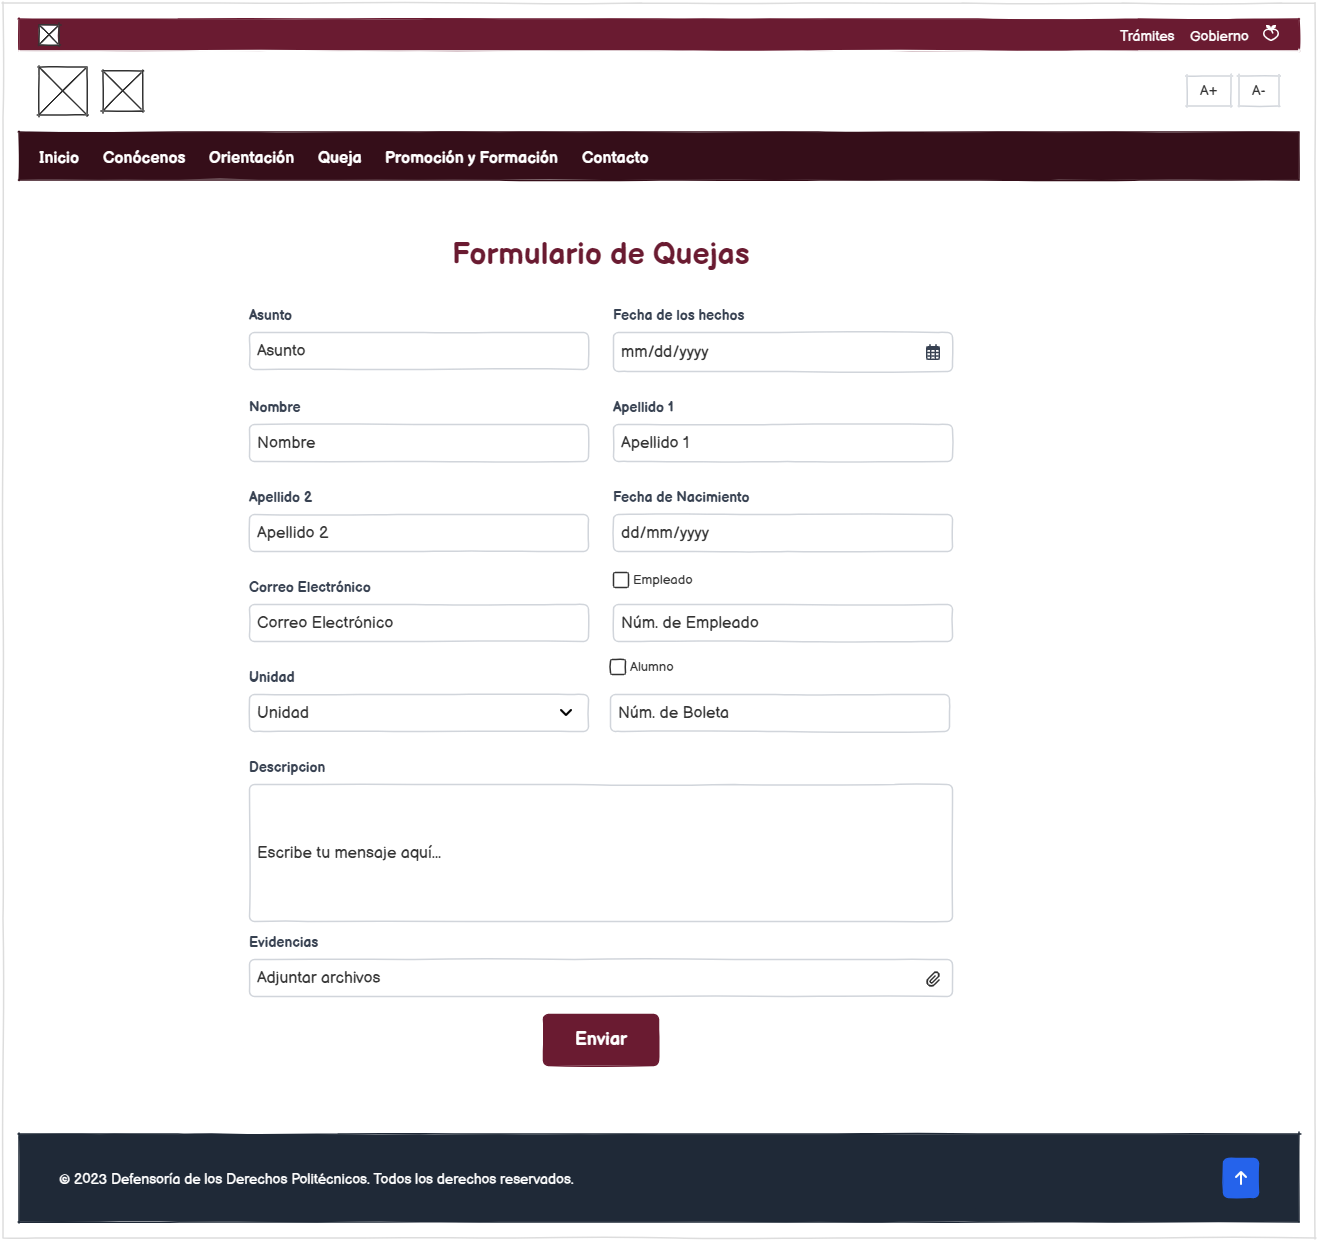
\includegraphics[width=0.65\textwidth]{imagenes/quejoso/FormularioQueja.png}
    \caption{MQ-02: Formulario para el registro de quejas.}
    \label{fig:mq02_formulario}
\end{figure}

\noindent \textbf{Descripción de la interfaz (MQ-02):} \\
Sobre esta interfaz presentamos el formulario a llenar para poder presentar una queja, abarcando aspecto importantes, como datos personales, datos de pertenencia al instituto, relato de los hechos, nombre del acusado y carga de evidencias, todo esto con el fin de poder crear una queja completamente valida.
\clearpage

% --- VISTA 03 ---
\begin{figure}[h]
    \centering
    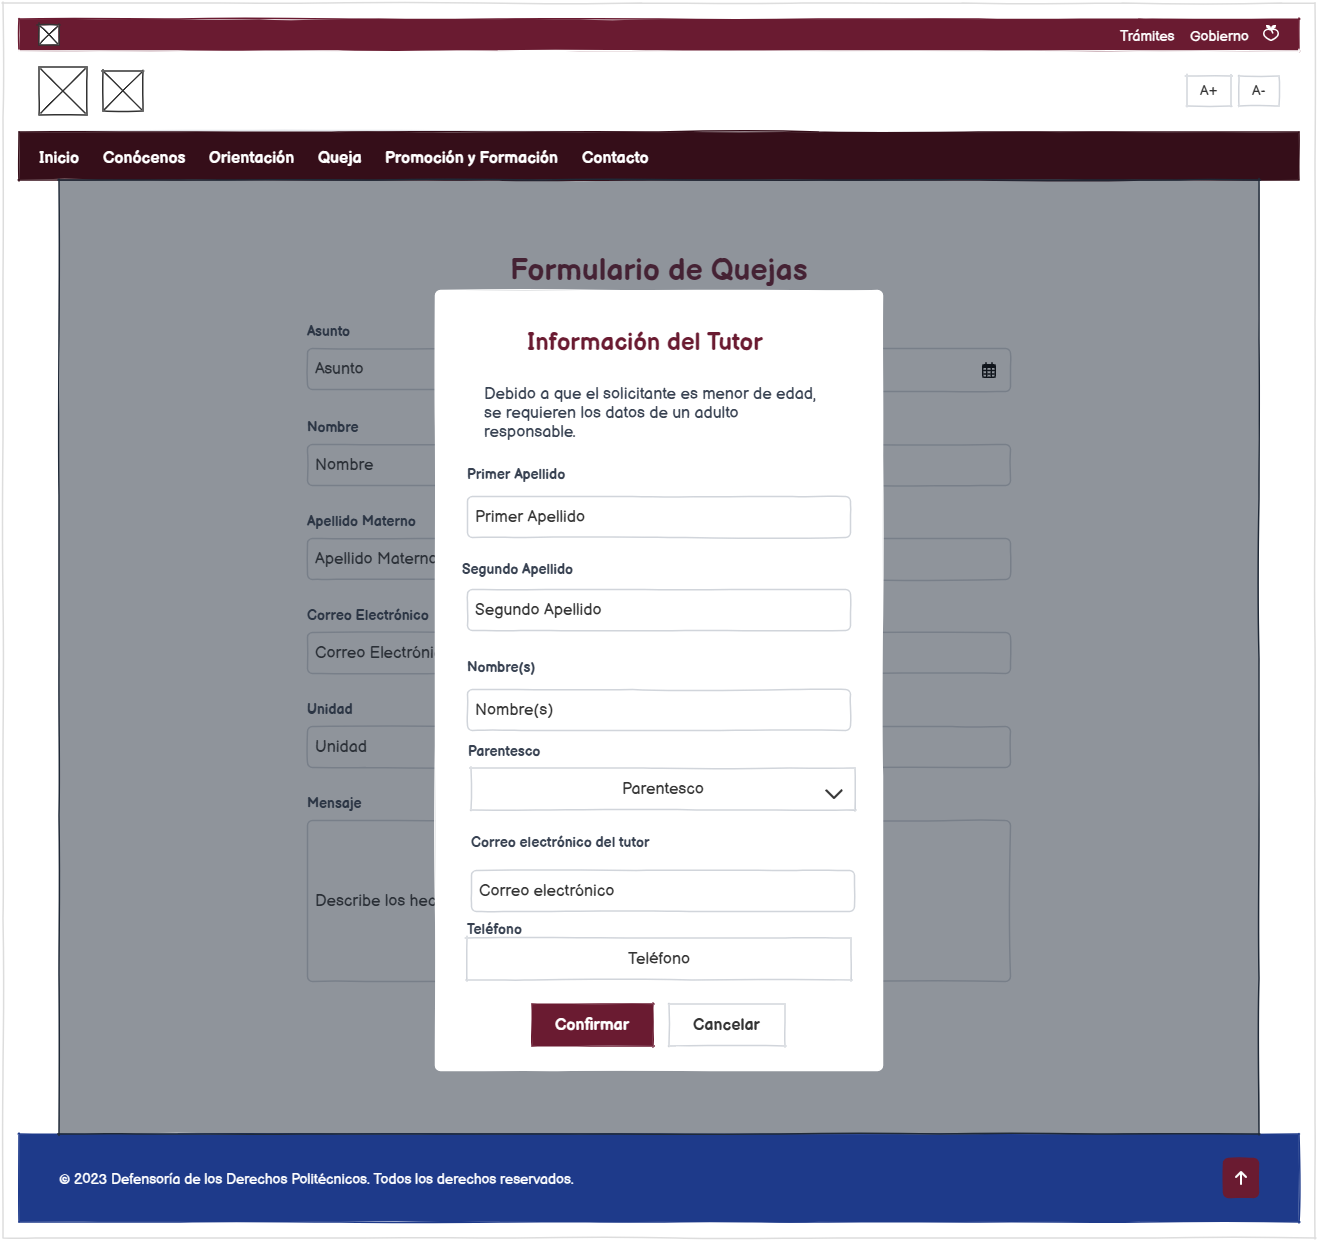
\includegraphics[width=0.75\textwidth]{imagenes/quejoso/FormularioTutor.png}
    \caption{MQ-03: Ventana emergente de información del tutor para menores de edad.}
    \label{fig:mq03_tutor}
\end{figure}

\noindent \textbf{Descripción de la interfaz (MQ-03):} \\
En dado caso de que el quejoso sea menor de edad, el conocimiento del tutor es indispensable, por ende, agregar los datos del mismo se vuelve fundamental para validar la queja, por ende, saldrá esta ventana  que permitira agregar los datos escenciales, como nombre, parentesco y medios de comunicación.

\clearpage %

% --- VISTA 04 ---
\begin{figure}[h]
    \centering
    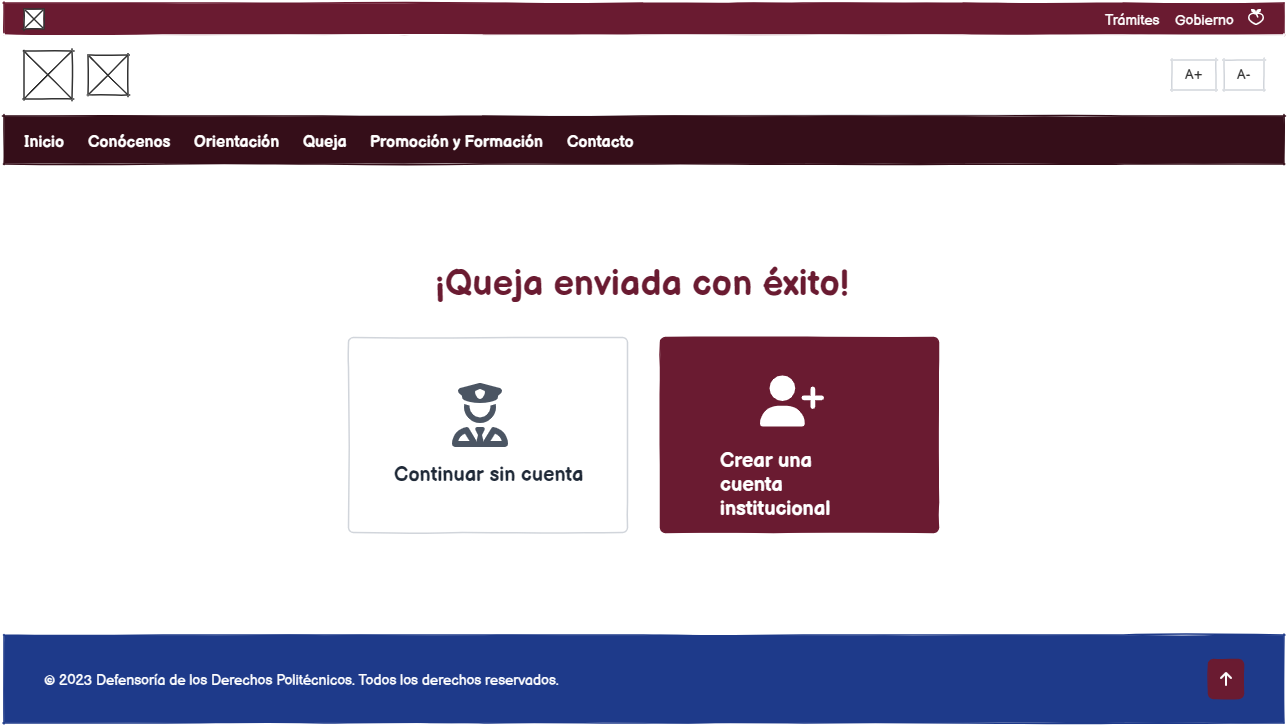
\includegraphics[width=0.65\textwidth]{imagenes/quejoso/QuejaEnviada.png}
    \caption{MQ-04: Pantalla de confirmación de envío exitoso.}
    \label{fig:mq04_exito}
\end{figure}

\noindent \textbf{Descripción de la interfaz (MQ-04):} \\
Una vez que el formulario es procesado correctamente, el sistema despliega esta pantalla de confirmación que asegura al usuario la recepción de su trámite y le permite elegir entre continuar sin cuenta o crear una cuenta dentro de la defonsoría para que el mismo quejoso pueda llevar un control de todas sus quejas.



% --- VISTA 05 ---
\begin{figure}[h]
    \centering
    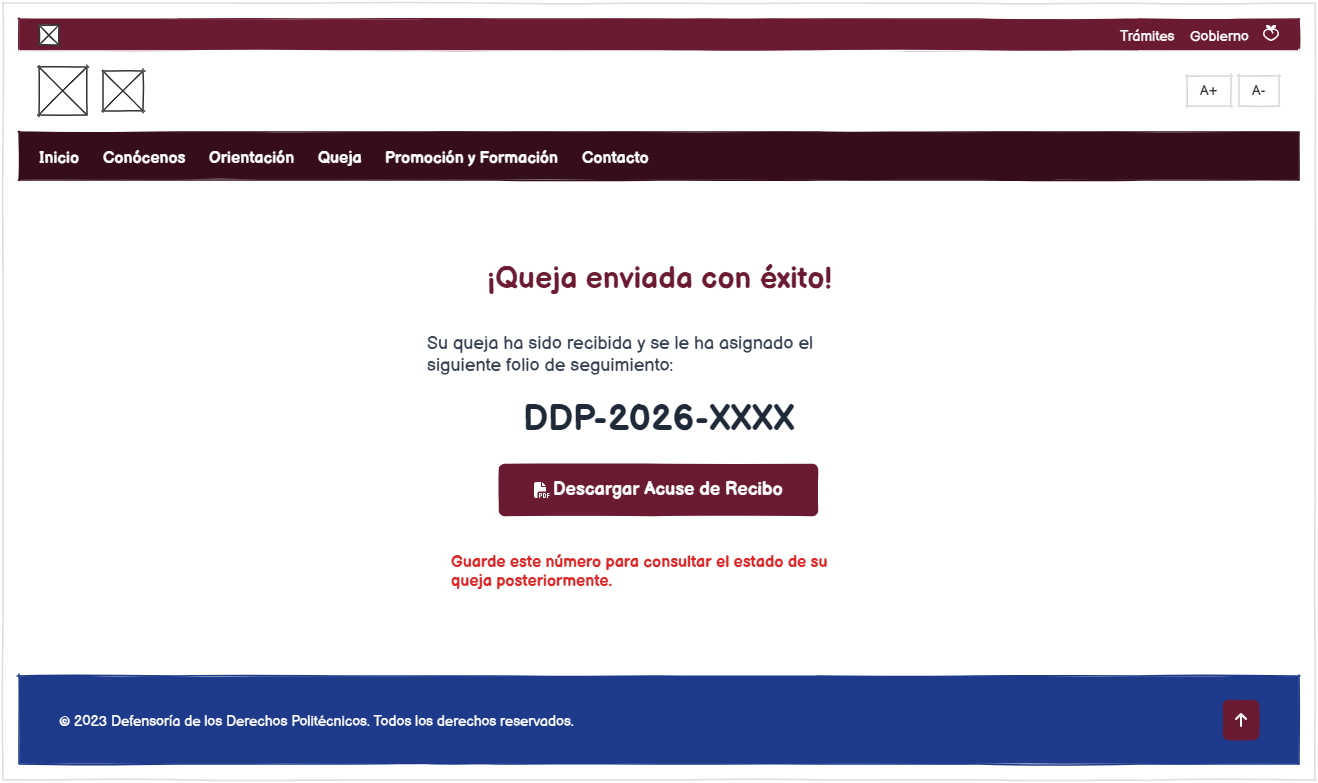
\includegraphics[width=0.65\textwidth]{imagenes/quejoso/FolioSeguimiento_NoCrearCuenta.png}
    \caption{MQ-05: Pantalla de finalización para usuarios sin registro de cuenta.}
    \label{fig:mq05_folio_sin_cuenta}
\end{figure}

\noindent \textbf{Descripción de la interfaz (MQ-05):} \\
Al seleccionar continuar sin cuenta, observamos la gneración de folio, y la opción de descargar el PDF que contiene el mismo.


% --- VISTA 06 ---
\begin{figure}[h]
\centering
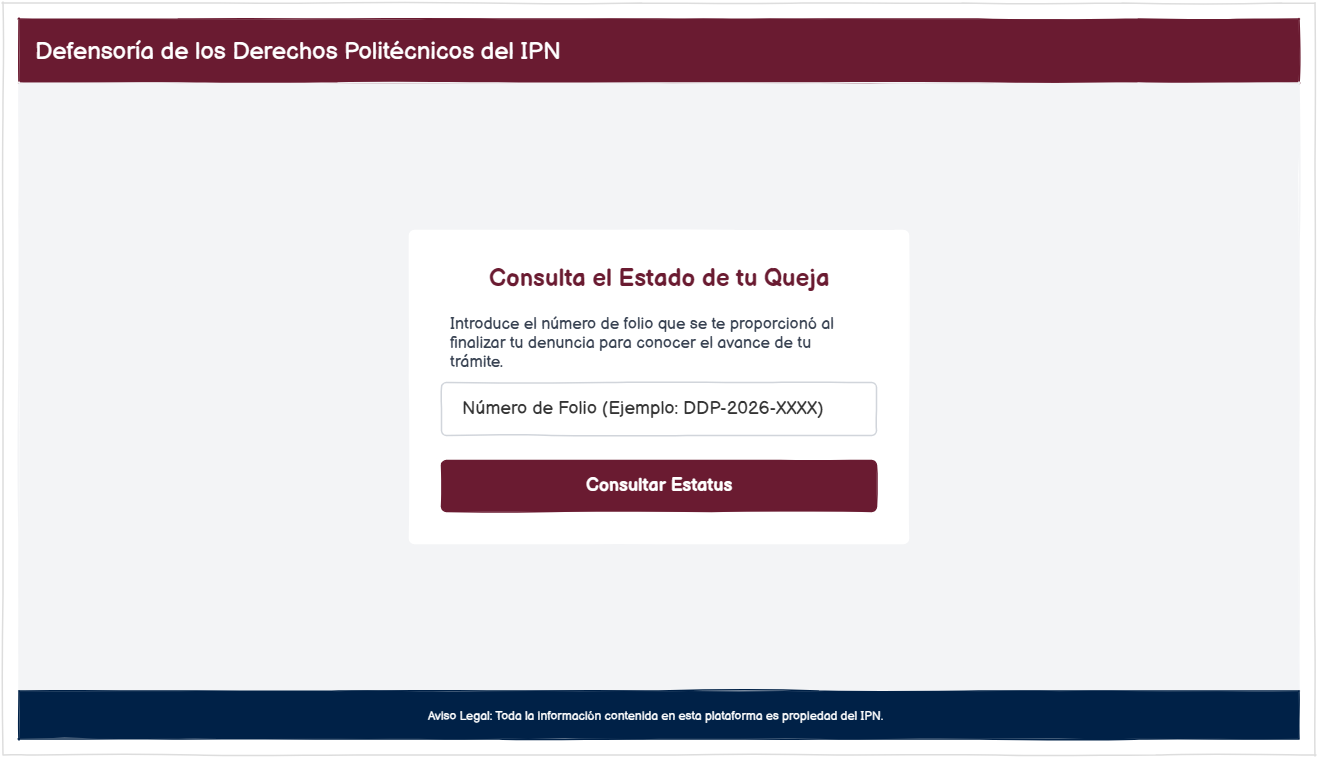
\includegraphics[width=0.65\textwidth]{imagenes/quejoso/ConsultaEstadoQueja.png}
\caption{MQ-06: Interfaz de consulta de estado mediante folio.}
\label{fig:mq06_consulta_folio}
\end{figure}

\noindent \textbf{Descripción de la interfaz (MQ-06):} \
Esta interfaz está diseñada para aquellos usuarios que optaron por no crear una cuenta pero desean conocer el avance de su trámite de manera rápida. Es una pantalla simple y directa que se centra en la recuperación de información mediante el folio asignado previamente por el sistema.

Presentamos un campo de entrada principal donde el quejoso debe ingresar su número de folio institucional y un botón de acción para realizar la consulta. Al ser una vía de acceso veloz, se eliminan distractores visuales, manteniendo únicamente la identidad gráfica del instituto y un enlace de ayuda en caso de que el usuario haya extraviado su código de seguimiento.

\vspace{1cm}

% --- VISTA 07 ---
\begin{figure}[h]
\centering
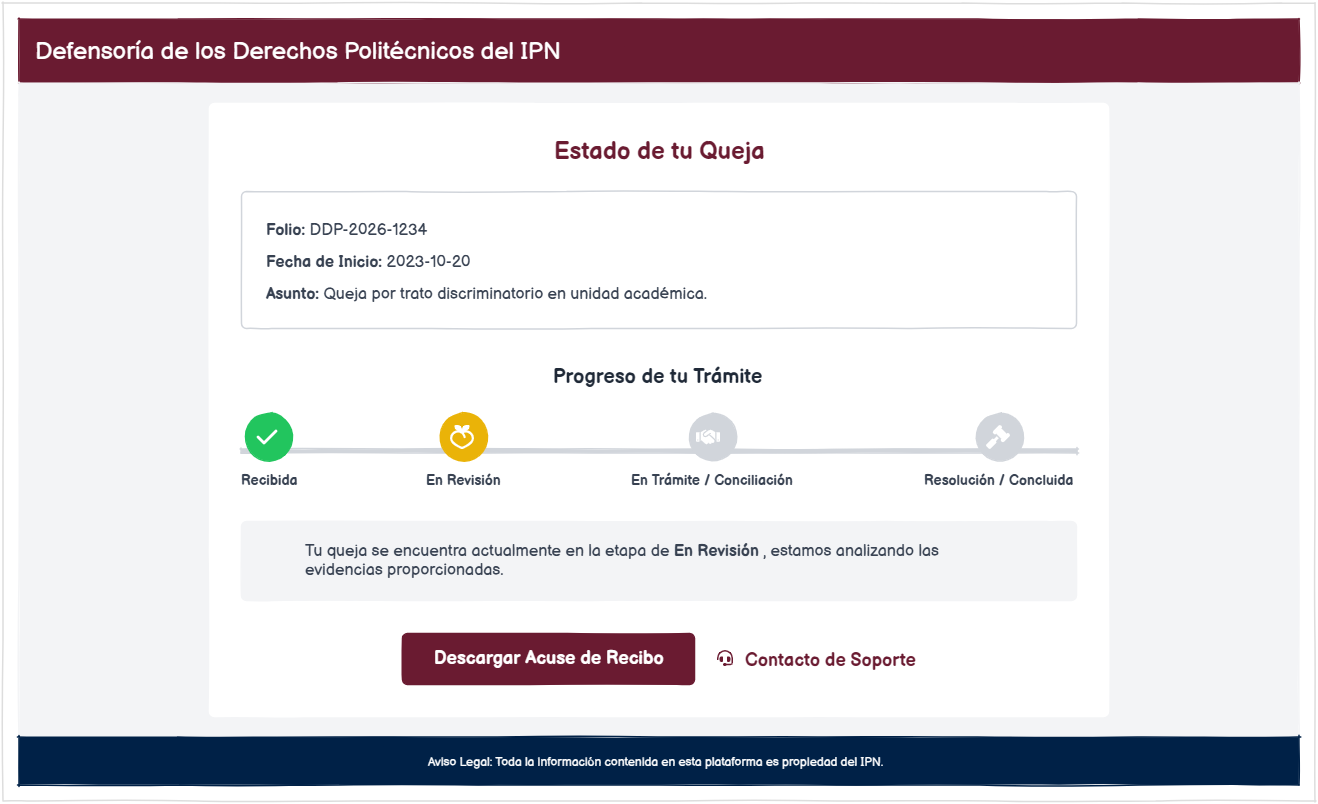
\includegraphics[width=0.65\textwidth]{imagenes/quejoso/EstadoQueja.png}
\caption{MQ-07: Pantalla de visualización del estado y progreso del trámite.}
\label{fig:mq07_estado_progreso}
\end{figure}

\noindent \textbf{Descripción de la interfaz (MQ-07):} \
Esta pantalla proporciona una visión detallada y actualizada del estatus de una queja específica, con un diseño orientado a reducir la incertidumbre del usuario sobre su proceso. La interfaz presenta un resumen del expediente mediante un recuadro informativo que muestra datos clave como el folio, la fecha de inicio y un asunto breve, permitiendo confirmar la identidad del trámite de manera inmediata.

Para facilitar la comprensión del avance, se incluye una línea de tiempo de progreso que sirve como indicador visual de los pasos administrativos, desde la recepción hasta la resolución final. Este componente se complementa con un mensaje de estatus detallado que explica de forma clara la situación actual de la queja, humanizando la interacción técnica. Finalmente, se habilitan acciones de usuario para descargar el acuse de recibo oficial o acceder a un contacto de soporte para resolver dudas adicionales.



% --- VISTA 08 ---
\begin{figure}[h]
\centering
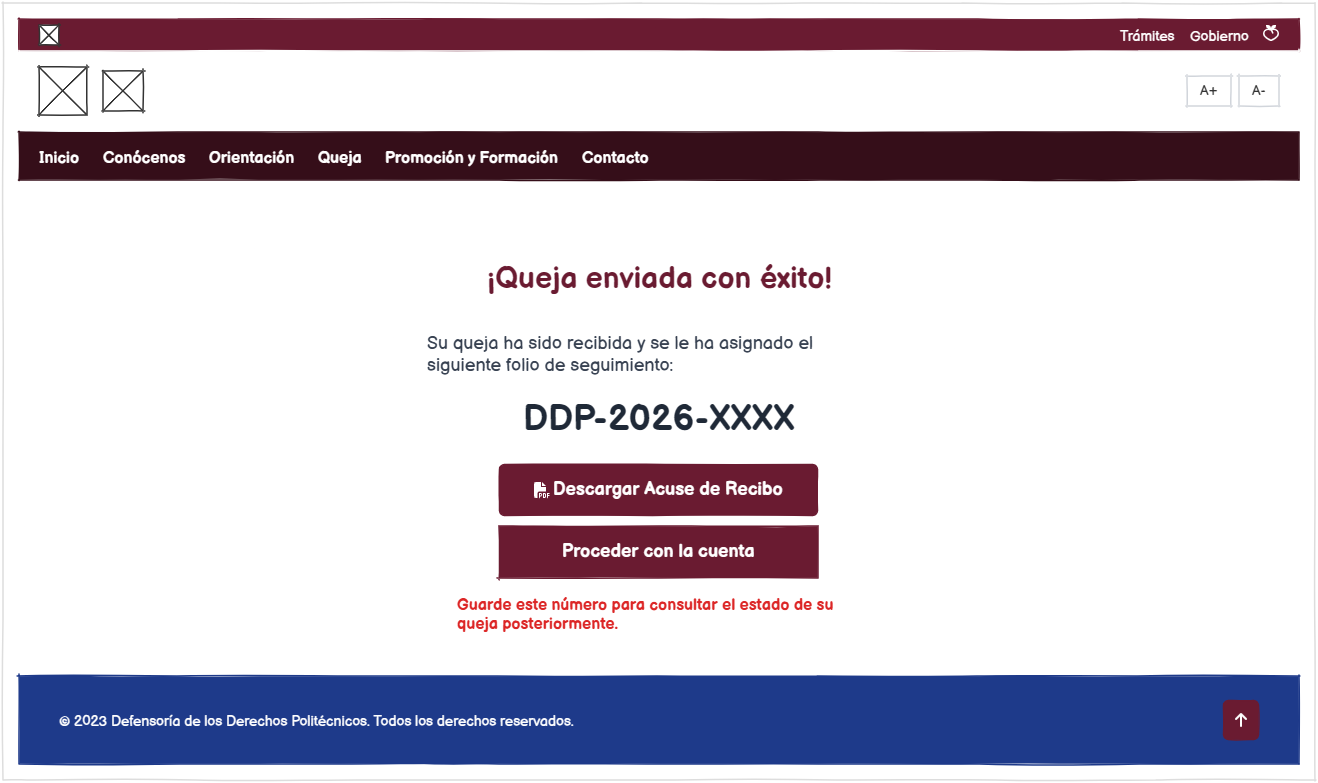
\includegraphics[width=0.65\textwidth]{imagenes/quejoso/FolioSeguimiento_CrearCuenta.png}
\caption{MQ-08: Pantalla de asignación de folio y creación de cuenta.}
\label{fig:mq08_folio}
\end{figure}

\noindent \textbf{Descripción de la interfaz (MQ-08):} \
Esta pantalla es fundamental para la transparencia del proceso, ya que proporciona al usuario la clave única para consultar el estado de su trámite en el futuro. A diferencia de otras vistas de finalización, esta versión está orientada específicamente a los usuarios que sí desean formalizar un registro en la plataforma para gestionar sus quejas de forma centralizada.

Se muestra de forma prominente el folio de seguimiento alfanumérico que servirá como referencia legal para el quejoso. Asimismo, se incluye un botón para descargar el acuse de recibo en formato PDF y un botón de transición que dirige al usuario al flujo de configuración de su perfil institucional, acompañado de una nota de advertencia sobre la importancia de resguardar estos datos.

\clearpage


% --- VISTA 09 ---
\begin{figure}[h]
\centering
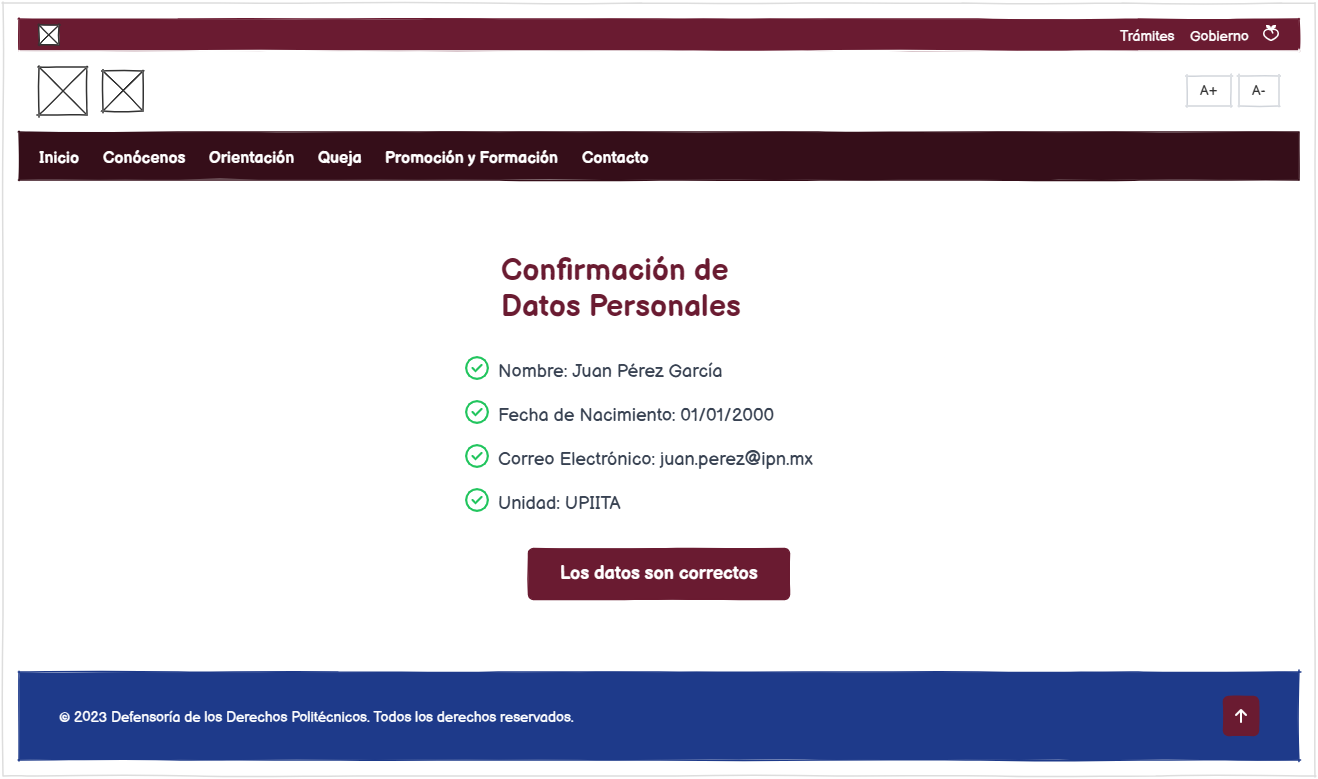
\includegraphics[width=0.65\textwidth]{imagenes/quejoso/ConfiguraciónDatosPersonales_CrearCuenta.png}
\caption{MQ-09: Pantalla de confirmación de datos personales para registro.}
\label{fig:mq09_confirmacion_datos}
\end{figure}

\noindent \textbf{Descripción de la interfaz (MQ-09):} \
Tras optar por la creación de una cuenta institucional, el sistema presenta esta vista de verificación de identidad. El objetivo principal es asegurar la integridad de la información que quedará vinculada permanentemente al nuevo perfil del usuario antes de proceder con el alta en la base de datos.

La interfaz presenta un resumen de identidad con los datos capturados anteriormente, como el nombre completo y la fecha de nacimiento, resaltando la vinculación institucional mediante el correo electrónico y la unidad académica perteneciente al IPN. Un botón de validación final permite al usuario confirmar que los datos son correctos, manteniendo un diseño minimalista que enfoca la atención en la revisión de la información.



% --- VISTA 10 ---
\begin{figure}[h]
\centering
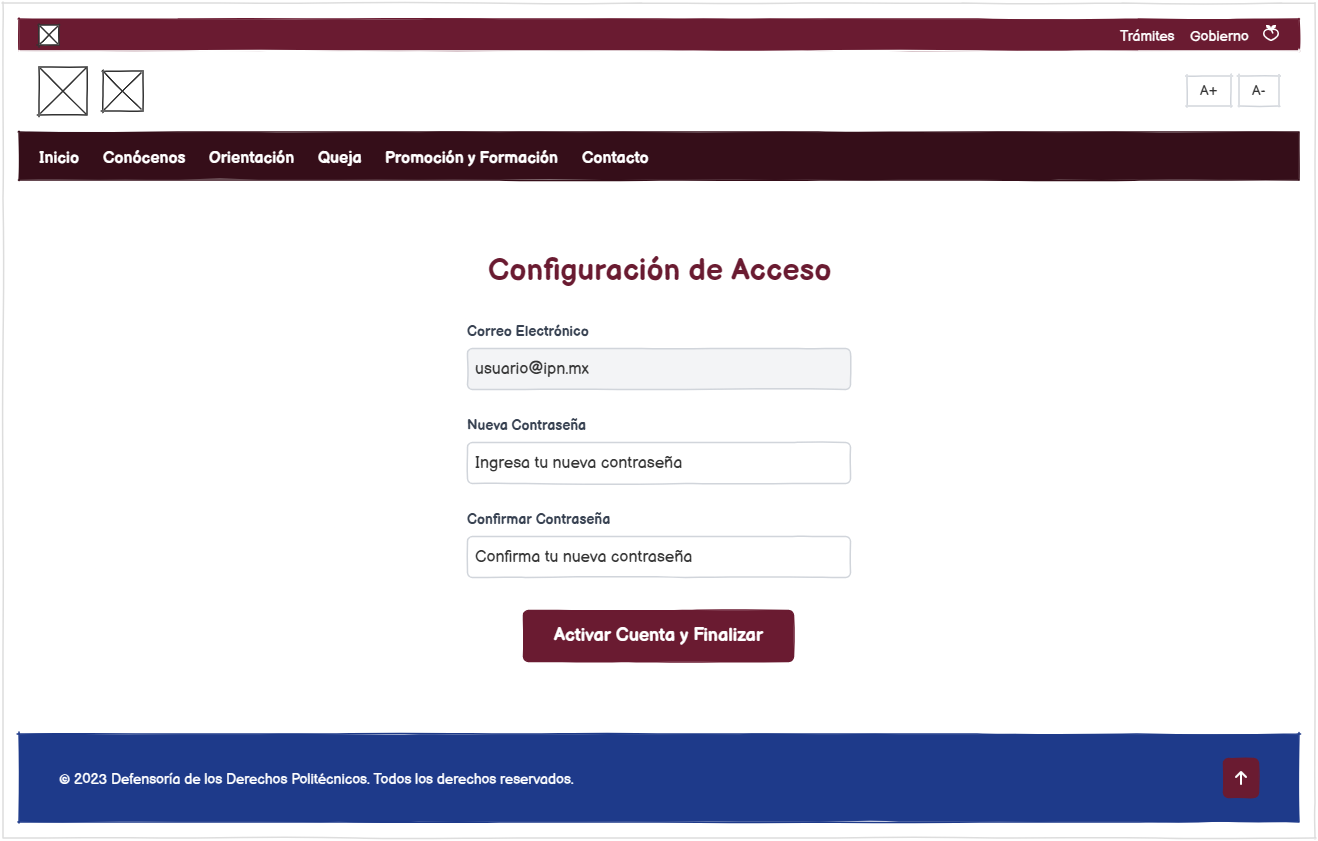
\includegraphics[width=0.65\textwidth]{imagenes/quejoso/ConfiguraciónAcceso_CrearCuenta.png}
\caption{MQ-10: Pantalla de configuración de acceso y seguridad.}
\label{fig:mq10_configuracion_acceso}
\end{figure}

\noindent \textbf{Descripción de la interfaz (MQ-10):} \
Esta vista finaliza el proceso de registro mediante el establecimiento de las credenciales de seguridad del usuario. La interfaz se enfoca exclusivamente en la protección de la cuenta y la configuración del acceso personal al portal de la defensoría.

En esta pantalla se muestra el identificador de usuario, que corresponde al correo electrónico institucional, y se habilitan campos con máscara de seguridad para la creación y confirmación de la contraseña. Al presionar el botón de activación, el sistema completa la transacción, vinculando formalmente la queja que originó el proceso con el nuevo perfil de usuario creado, permitiendo el acceso inmediato al tablero de control.


% --- VISTA 11 ---
\begin{figure}[h]
\centering
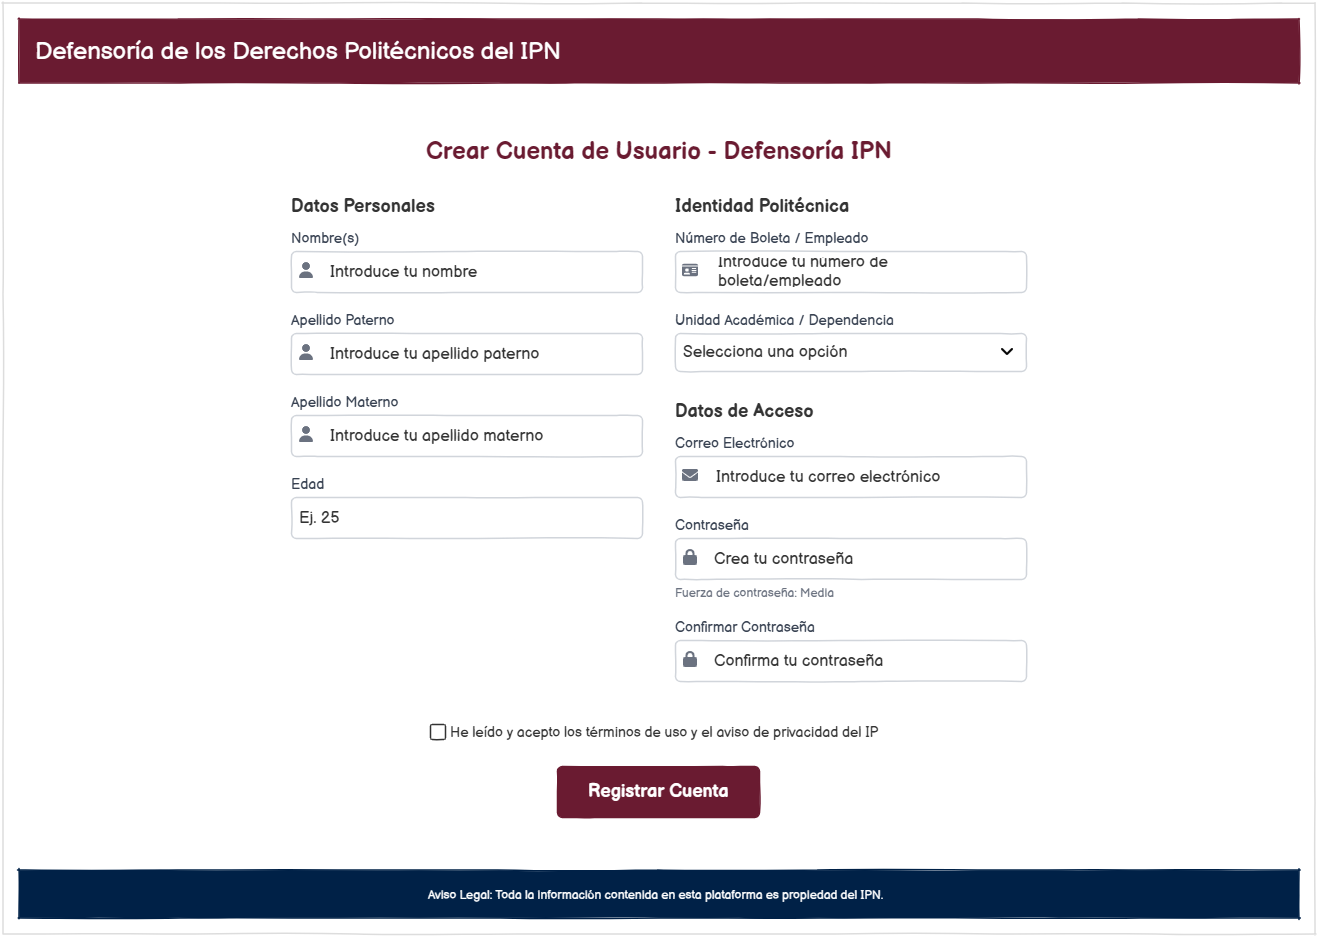
\includegraphics[width=0.65\textwidth]{imagenes/quejoso/CrearCuenta_Quejoso.png}
\caption{MQ-11: Formulario general de creación de cuenta de usuario.}
\label{fig:mq11_registro_general}
\end{figure}

\noindent \textbf{Descripción de la interfaz (MQ-11):} \
Esta interfaz permite a cualquier miembro de la comunidad politécnica dar de alta un perfil en la plataforma de manera independiente. El formulario está organizado de forma lógica para facilitar la captura de datos personales como nombre y edad, así como la identidad politécnica mediante el número de boleta o empleado y la unidad académica.

Para garantizar la seguridad, la pantalla incluye la configuración del correo y una contraseña con indicadores visuales de robustez. Finalmente, se integra un apartado para la aceptación de términos y el aviso de privacidad institucional, permitiendo que el registro sea válido bajo la normativa del instituto.

\clearpage


% --- VISTA 12 ---
\begin{figure}[h]
\centering
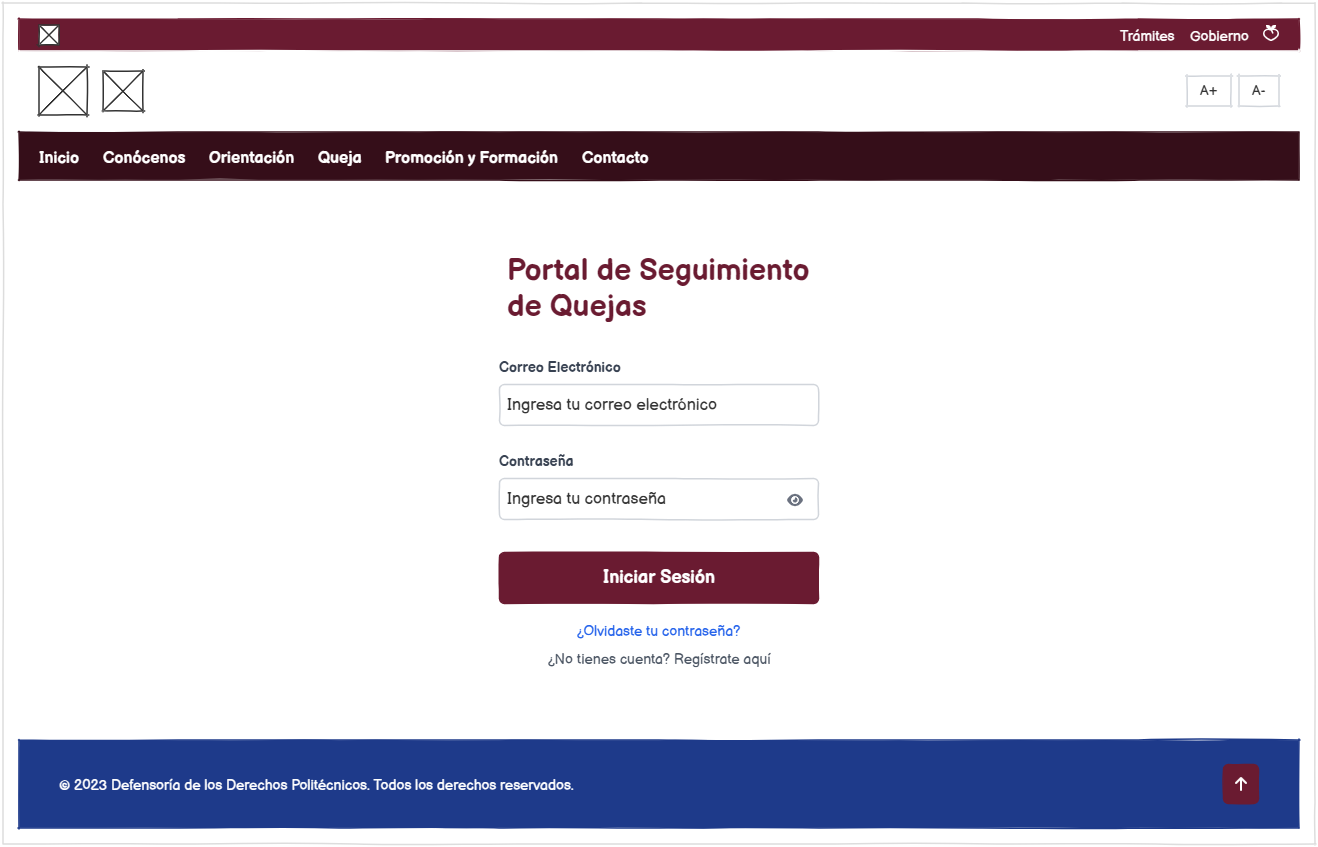
\includegraphics[width=0.65\textwidth]{imagenes/quejoso/InicioSesion_Quejoso.png}
\caption{MQ-12: Interfaz de inicio de sesión para el portal de seguimiento.}
\label{fig:mq12_login}
\end{figure}

\noindent \textbf{Descripción de la interfaz (MQ-12):} \
Esta interfaz representa el punto de acceso para los usuarios que ya cuentan con un registro previo. Está diseñada para ser directa, solicitando únicamente el correo electrónico y la contraseña, la cual cuenta con un icono de visibilidad para evitar errores durante la captura.

En la parte inferior del bloque de acceso, se proporcionan enlaces de apoyo para la recuperación de contraseña o para redirigir a nuevos usuarios al formulario de registro. El diseño conserva el encabezado institucional completo, permitiendo que el usuario navegue hacia las secciones informativas de la defensoría antes de autenticarse.



% --- VISTA 13 ---
\begin{figure}[h]
\centering
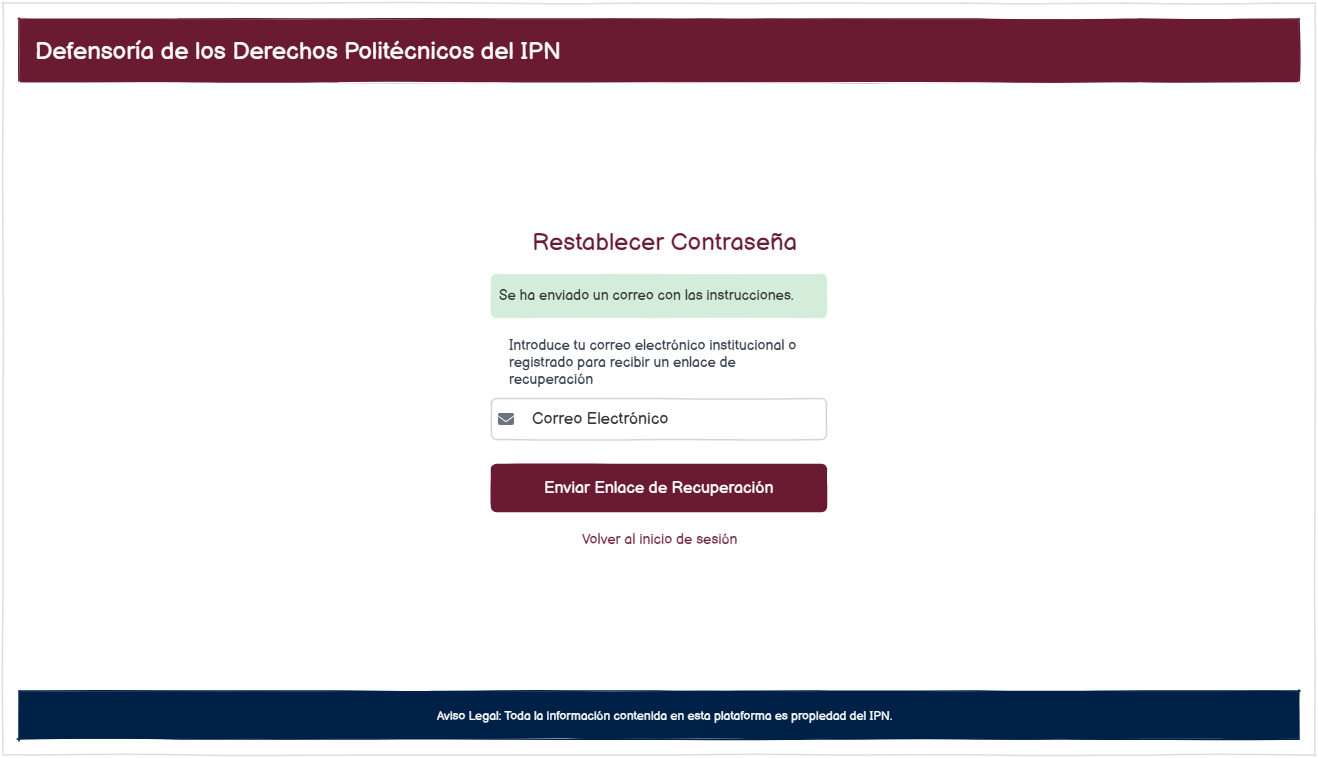
\includegraphics[width=0.65\textwidth]{imagenes/quejoso/RecuperarContraseña_Quejoso.png}
\caption{MQ-13: Interfaz de restablecimiento de contraseña.}
\label{fig:mq13_recuperar_pass}
\end{figure}

\noindent \textbf{Descripción de la interfaz (MQ-13):} \
Esta vista proporciona un mecanismo de autoservicio para los usuarios que han perdido el acceso a su cuenta, centrando la interacción en un proceso de recuperación simple. El sistema solicita el correo electrónico registrado para enviar un enlace seguro de restablecimiento.

Una característica clave de esta interfaz es la retroalimentación visual mediante una alerta que confirma el envío exitoso de las instrucciones. Además, se incluye un enlace de retorno al inicio de sesión para facilitar la navegación en caso de que el usuario acceda a esta pantalla por error, manteniendo siempre la limpieza visual y el enfoque en una sola tarea.



% --- VISTA 14 ---
\begin{figure}[h]
\centering
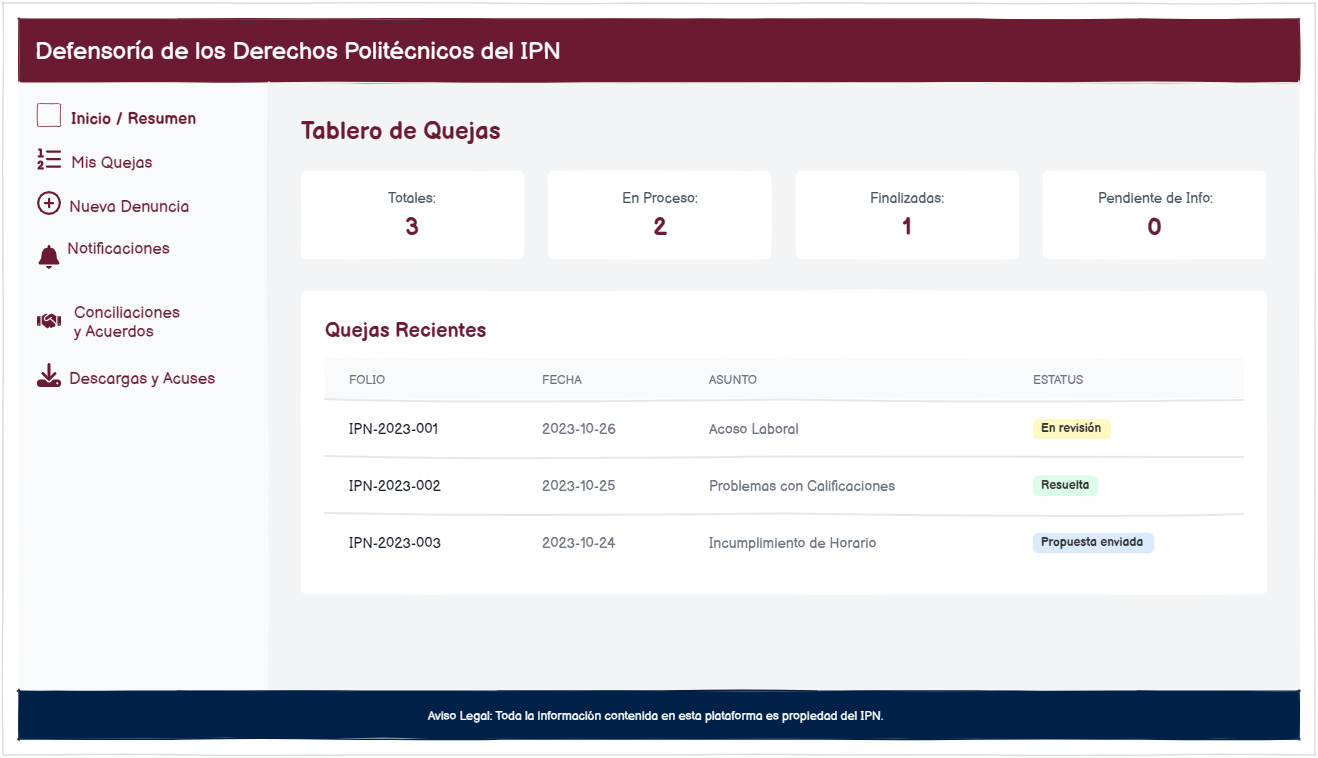
\includegraphics[width=0.65\textwidth]{imagenes/quejoso/Dashboard_Quejoso.png}
\caption{MQ-14: Tablero de control principal del usuario registrado.}
\label{fig:mq14_dashboard}
\end{figure}

\noindent \textbf{Descripción de la interfaz (MQ-14):} \
Esta pantalla constituye el centro de mando del quejoso una vez iniciada la sesión, ofreciendo un resumen ejecutivo de todos sus trámites. A través de un menú lateral, el usuario puede navegar entre sus quejas, realizar nuevas denuncias o revisar notificaciones y documentos de conciliación de forma organizada.

El tablero destaca mediante tarjetas estadísticas el estado general de las solicitudes, permitiendo identificar rápidamente cuántas quejas están en proceso o finalizadas. Complementando esta información, se presenta una tabla detallada con los folios recientes, sus fechas y estatus específicos, lo que garantiza un control total sobre el seguimiento administrativo desde una sola vista.

\clearpage


% --- VISTA 15 ---
\begin{figure}[h]
\centering
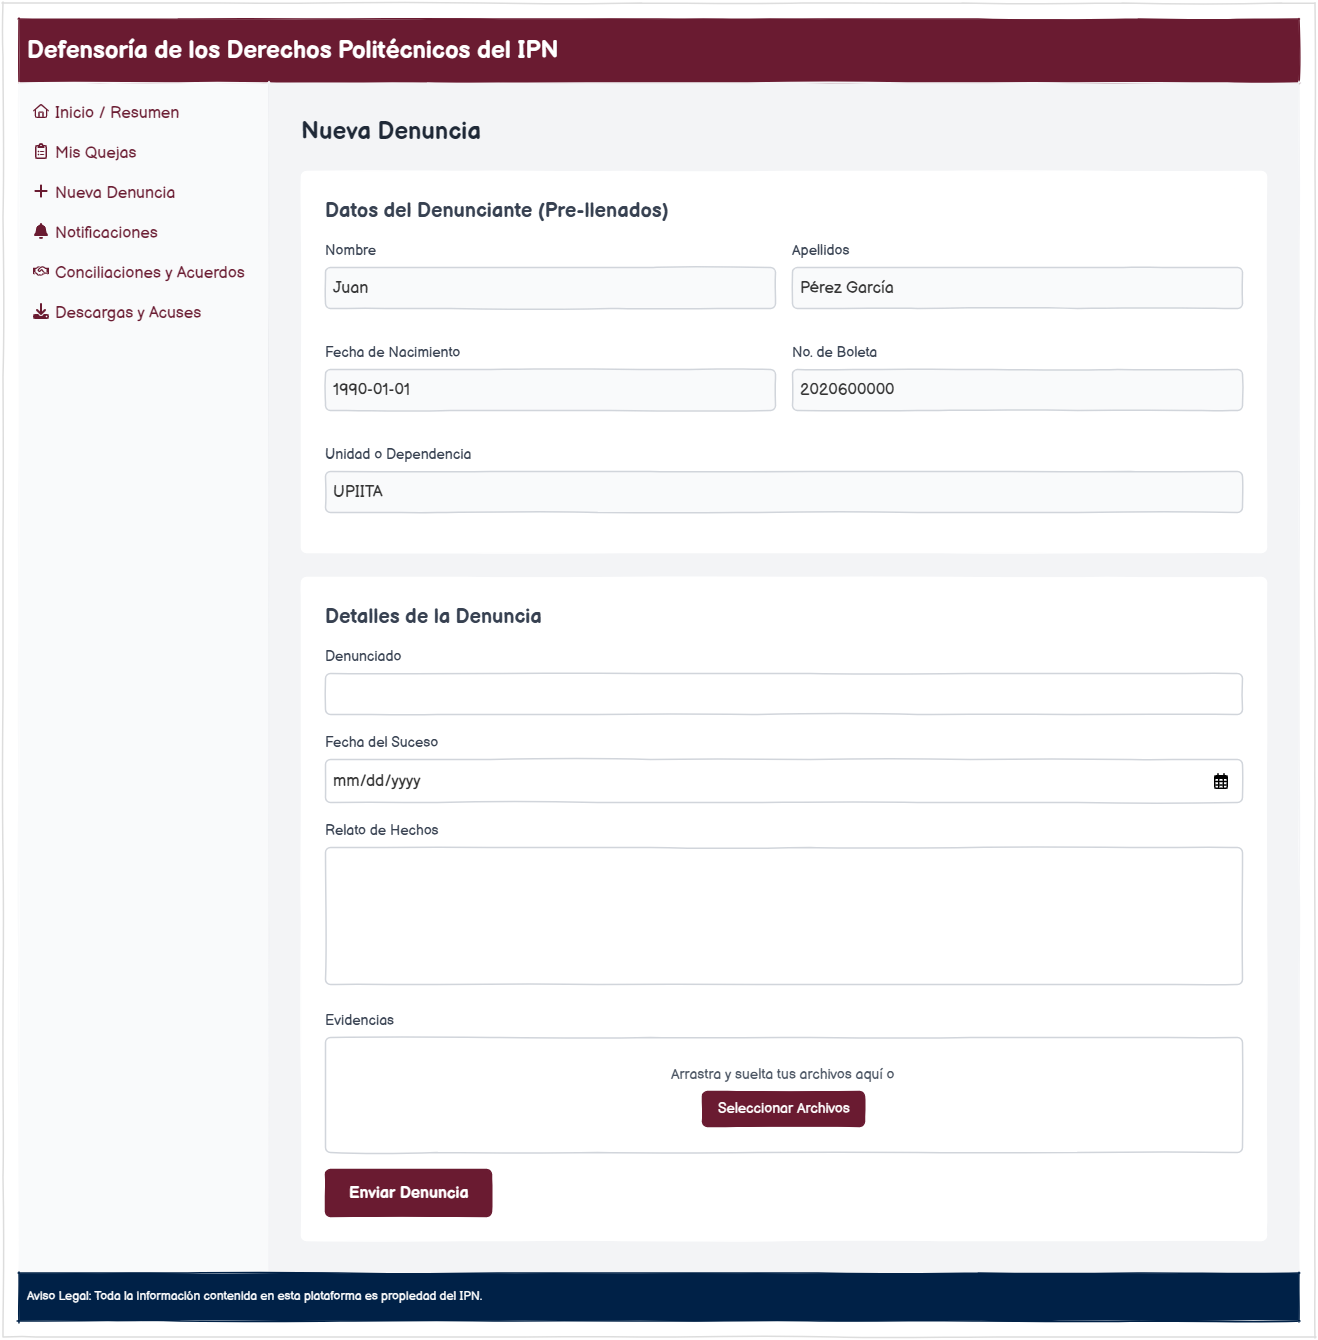
\includegraphics[width=0.65\textwidth]{imagenes/quejoso/NuevaQueja.png}
\caption{MQ-15: Formulario de nueva denuncia para usuario autenticado.}
\label{fig:mq15_nueva_queja_auth}
\end{figure}

\noindent \textbf{Descripción de la interfaz (MQ-15):} \
Esta interfaz representa la optimización del proceso de denuncia para usuarios con cuenta activa, agilizando el trámite al recuperar automáticamente la información del perfil. El sistema pre-llena los datos de identidad del denunciante, permitiendo que el usuario se enfoque exclusivamente en describir los hechos y señalar al acusado.

Además de los campos de texto para el relato, se integra un área de gestión de evidencias que facilita la carga de archivos multimedia o documentos probatorios. Al mantener el menú lateral del panel de control, el quejoso puede realizar la denuncia sin perder la consistencia visual del sistema, asegurando una experiencia de usuario fluida y profesional.

\clearpage


% --- VISTA 16 ---
\begin{figure}[h]
\centering
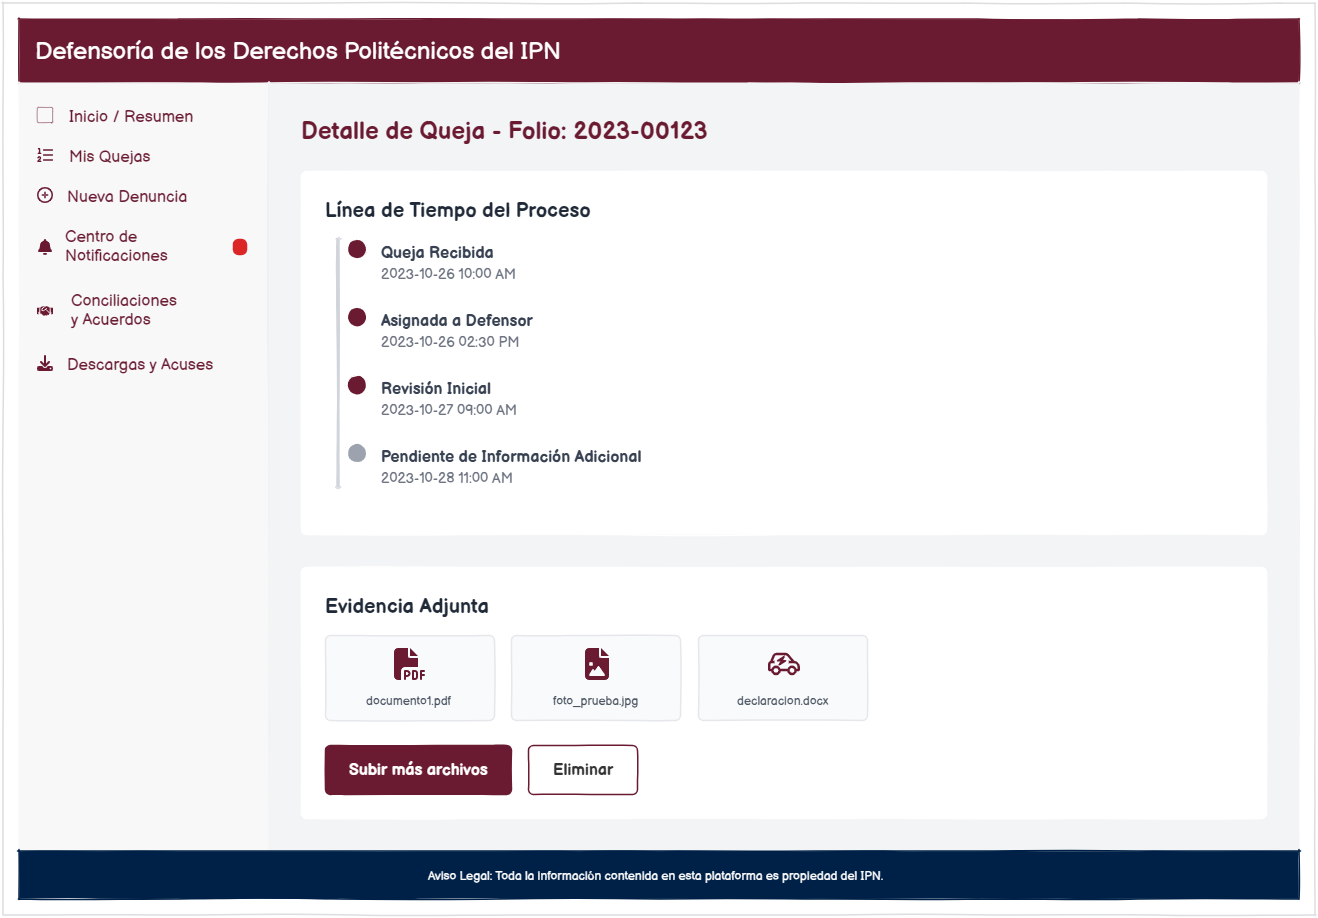
\includegraphics[width=0.65\textwidth]{imagenes/quejoso/DetallesyEvidenciaQujea.png}
\caption{MQ-16: Detalle de expediente con línea de tiempo y gestión de evidencias.}
\label{fig:mq16_detalle_evidencias}
\end{figure}

\noindent \textbf{Descripción de la interfaz (MQ-16):} \
Esta pantalla permite al usuario profundizar en el estado de una queja en particular, ofreciendo una auditoría clara del flujo de trabajo a través de una línea de tiempo vertical. En este historial se registran todos los hitos, desde la recepción hasta la asignación de un defensor, proporcionando transparencia absoluta sobre el avance del caso.

Junto a la cronología, se presenta un panel dedicado a la gestión de evidencias donde se listan todos los archivos adjuntos con iconos representativos de su formato. Esta sección otorga al usuario la posibilidad de subir documentación adicional en caso de ser requerida por la defensoría, manteniendo el expediente siempre actualizado y completo.



% --- VISTA 17 ---
\begin{figure}[h]
\centering
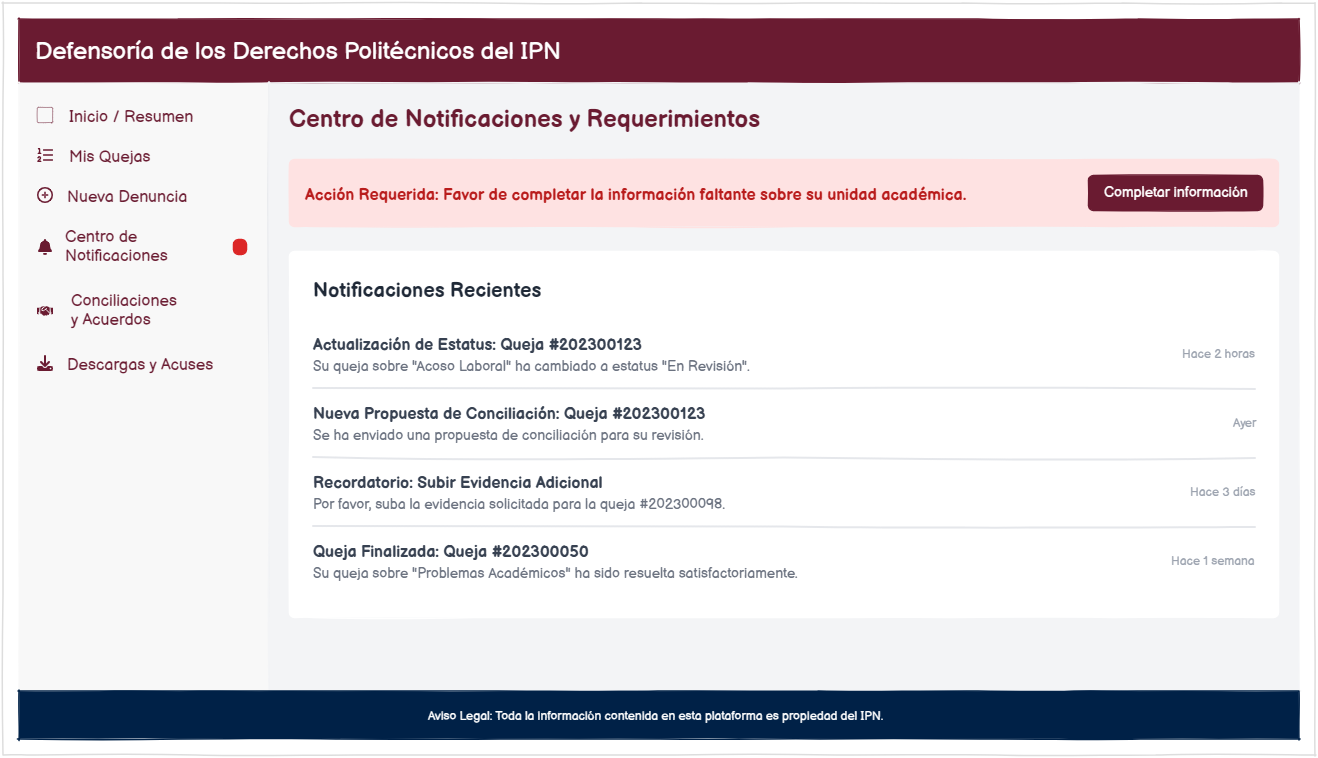
\includegraphics[width=0.65\textwidth]{imagenes/quejoso/NotificacionesRequerimientos.png}
\caption{MQ-17: Centro de notificaciones y gestión de requerimientos.}
\label{fig:mq17_notificaciones}
\end{figure}

\noindent \textbf{Descripción de la interfaz (MQ-17):} \
Esta pantalla centraliza las alertas y solicitudes de información, funcionando como el canal de comunicación oficial entre el sistema y el usuario. Se destaca un banner de acción requerida en la parte superior para señalar necesidades críticas, como la falta de datos específicos, permitiendo resolverlas mediante accesos directos.

El resto de la interfaz muestra un historial cronológico de eventos relevantes, permitiendo al usuario identificar la naturaleza de cada aviso, ya sean actualizaciones de estatus o propuestas de conciliación. El diseño asegura que ninguna solicitud administrativa pase desapercibida, utilizando indicadores visuales en el menú lateral que permanecen activos hasta que las notificaciones son atendidas.


% ------------------------------------------------------------------------------
% SECCIÓN 2: PERFIL ADMINISTRACIÓN Y DEFENSORÍA
% ------------------------------------------------------------------------------
\section{Perfil: Administración y Defensoría}
Este perfil integra las herramientas de gestión interna de la plataforma. El acceso está restringido al personal de la Defensoría de los Derechos Politécnicos y se divide en cuatro departamentos operativos con facultades diferenciadas para garantizar la debida atención de los expedientes.

% --- VISTA ADMINISTRATIVA 01 ---
\begin{figure}[h]
\centering
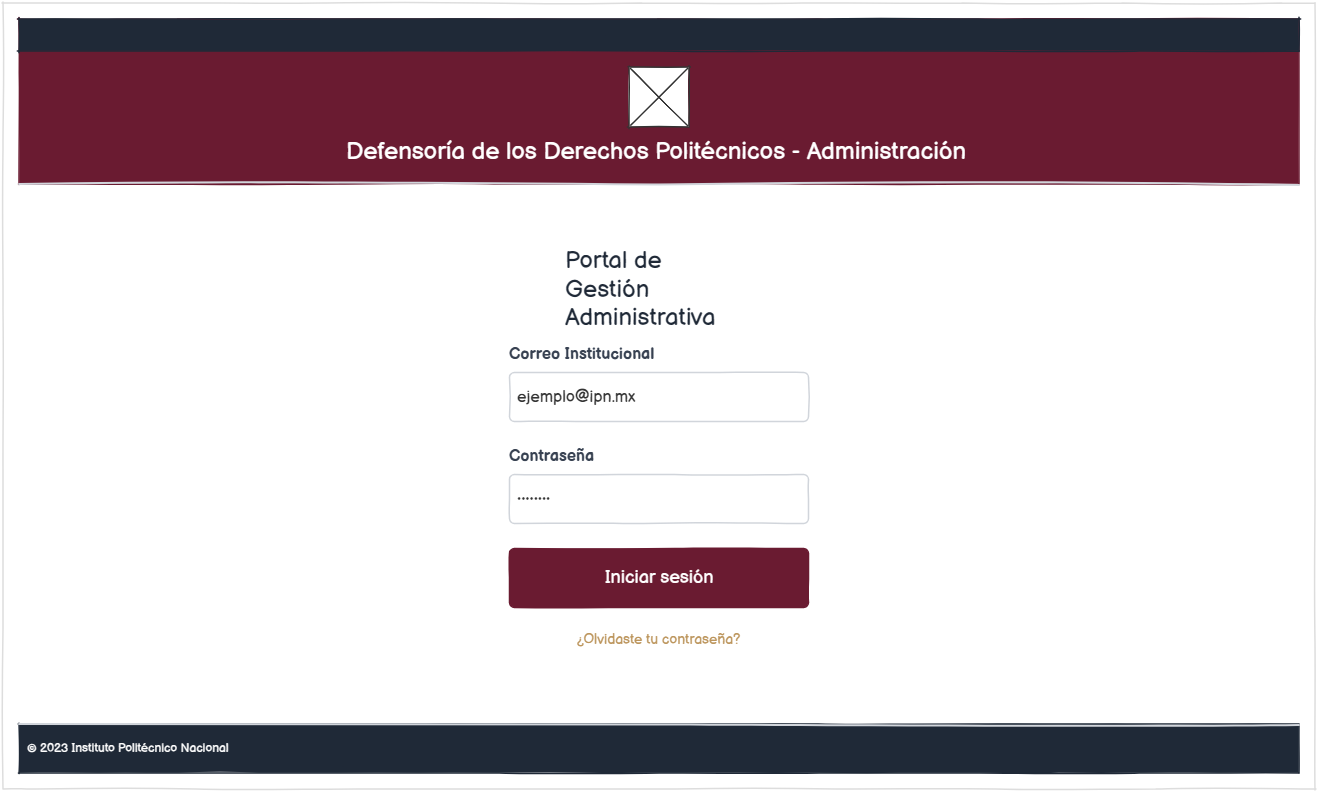
\includegraphics[width=0.65\textwidth]{imagenes/recepcion/InicioSesión_DDP.png}
\caption{MA-01: Portal de acceso al Sistema de Gestión Administrativa.}
\label{fig:ma01_login_adm}
\end{figure}

\noindent \textbf{Descripción de la interfaz (MA-01):} \
Esta interfaz representa el punto de acceso unificado para el personal de la Defensoría de los Derechos Politécnicos. A diferencia del portal ciudadano, esta vista está optimizada para la seguridad interna mediante un encabezado de administración que identifica claramente el módulo para evitar confusiones. El sistema presenta campos de credenciales vinculados al directorio institucional y un pie de página oficial que refuerza el carácter normativo del portal, permitiendo un acceso seguro y restringido a las funciones de gestión.


\clearpage

% --- VISTA ADMINISTRATIVA 02 ---
\begin{figure}[h]
\centering
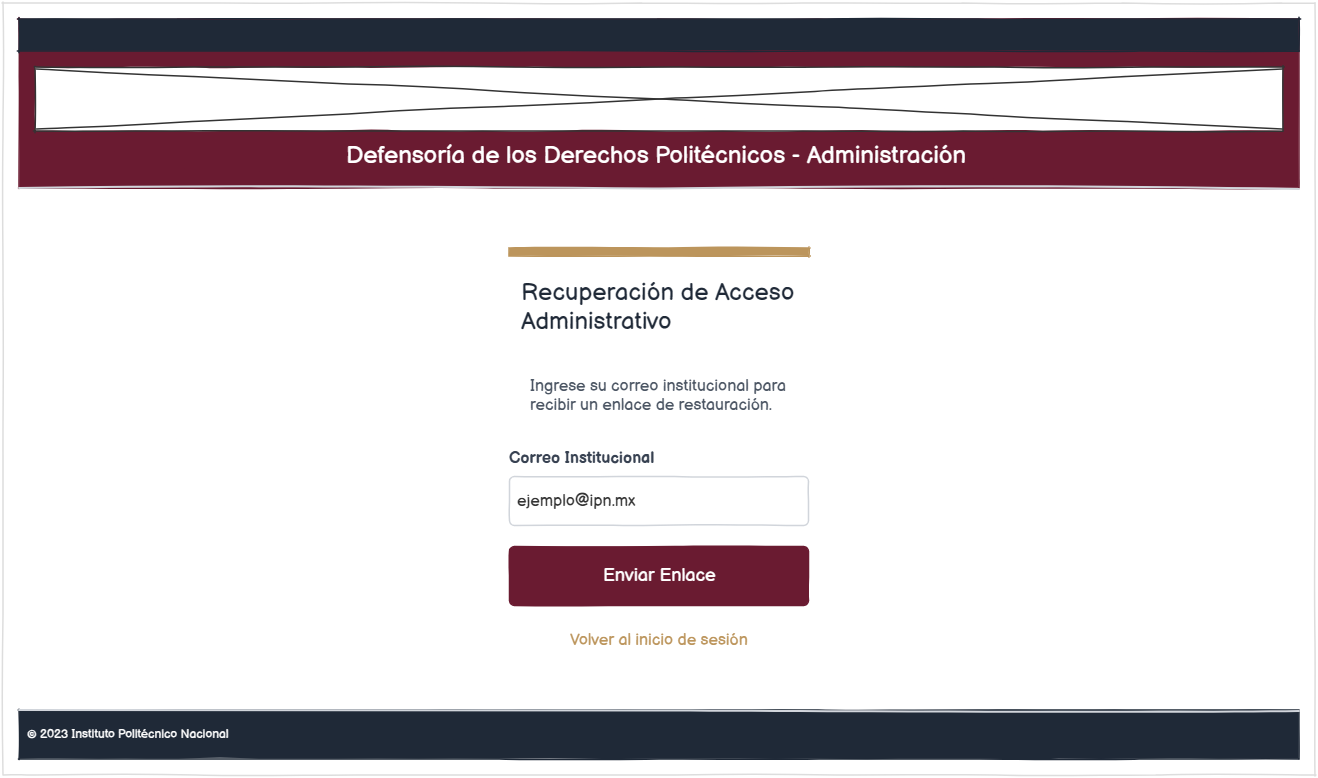
\includegraphics[width=0.65\textwidth]{imagenes/recepcion/RecuperaciónContraseñaDDP.png}
\caption{MA-02: Interfaz de recuperación de acceso para personal administrativo.}
\label{fig:ma02_recuperar_adm}
\end{figure}

\noindent \textbf{Descripción de la interfaz (MA-02):} \
Esta vista permite al personal de los cuatro departamentos restablecer sus credenciales de acceso de manera autónoma y segura. La validación institucional requiere exclusivamente el correo oficial para procesar la solicitud, asegurando que el enlace de restauración no sea desviado a cuentas externas. El flujo de recuperación cuenta con instrucciones directas y un control de navegación para volver al inicio de sesión, facilitando la recuperación del acceso sin comprometer la integridad del sistema administrativo.

\clearpage

\subsection{Departamento de Recepción}
Es el primer filtro del sistema, encargado de la validación inicial de los datos de entrada y la asignación preliminar de folios o turnos.

\begin{figure}[h]
\centering
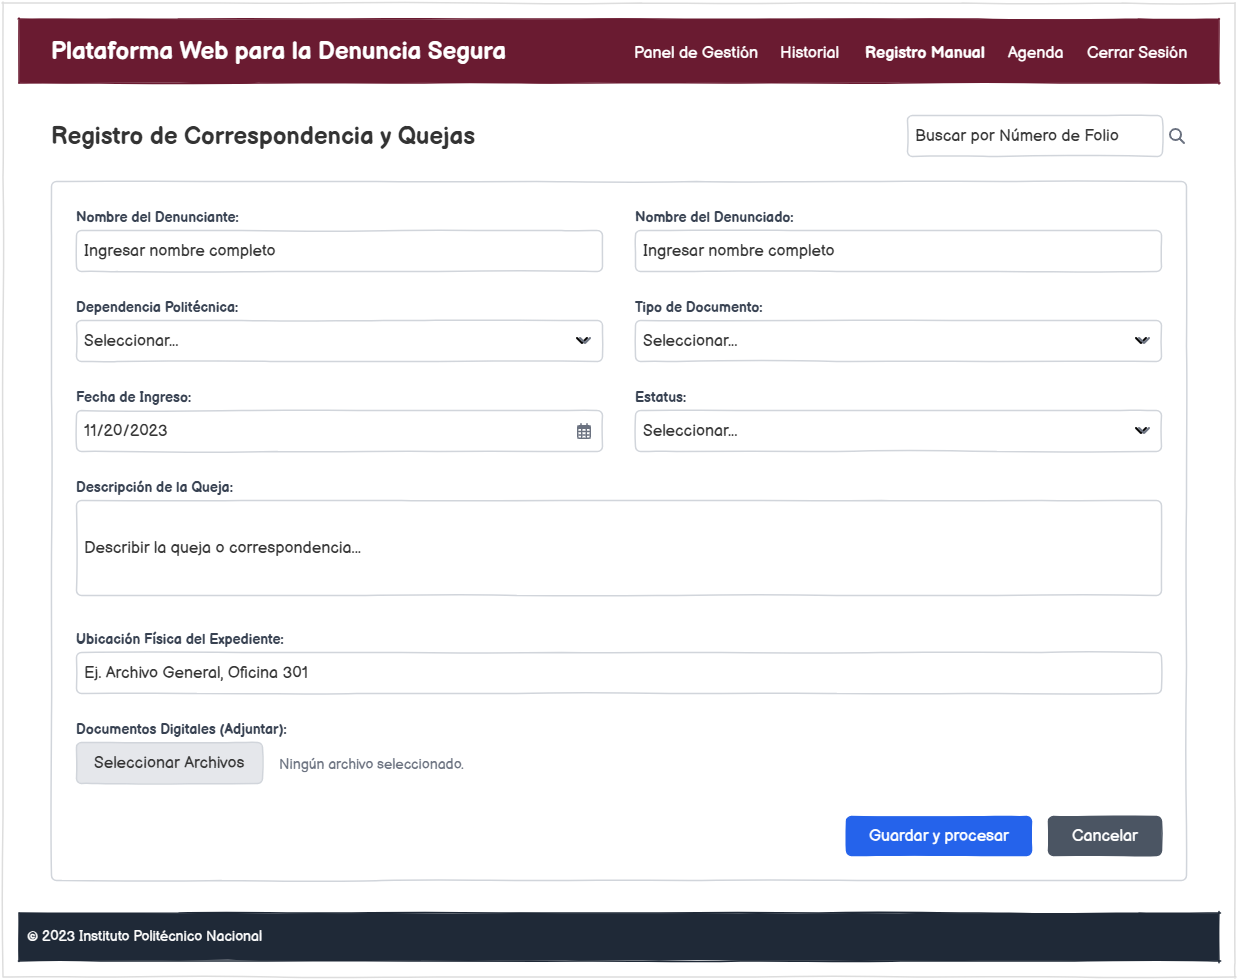
\includegraphics[width=0.65\textwidth]{imagenes/recepcion/RegistroManualQueja.png}
\caption{MA-03: Formulario de registro manual de correspondencia y quejas.}
\label{fig:ma03_registro_manual}
\end{figure}

\noindent \textbf{Descripción de la interfaz (MA-03):} \
Esta interfaz permite al personal administrativo registrar quejas o correspondencia recibida de manera presencial, facilitando la creación de un gemelo digital del expediente físico. La pantalla integra un buscador de folio para evitar duplicidad, campos para los datos de los sujetos involucrados y selectores para la clasificación administrativa y el estatus. Un elemento crítico es el campo especializado para registrar la ubicación del archivo físico, lo que garantiza la trazabilidad entre el papel original y el repositorio digital mediante la carga de evidencias escaneadas.


\clearpage

% --- VISTA 04: PANEL DE GESTIÓN ---
\begin{figure}[h]
\centering
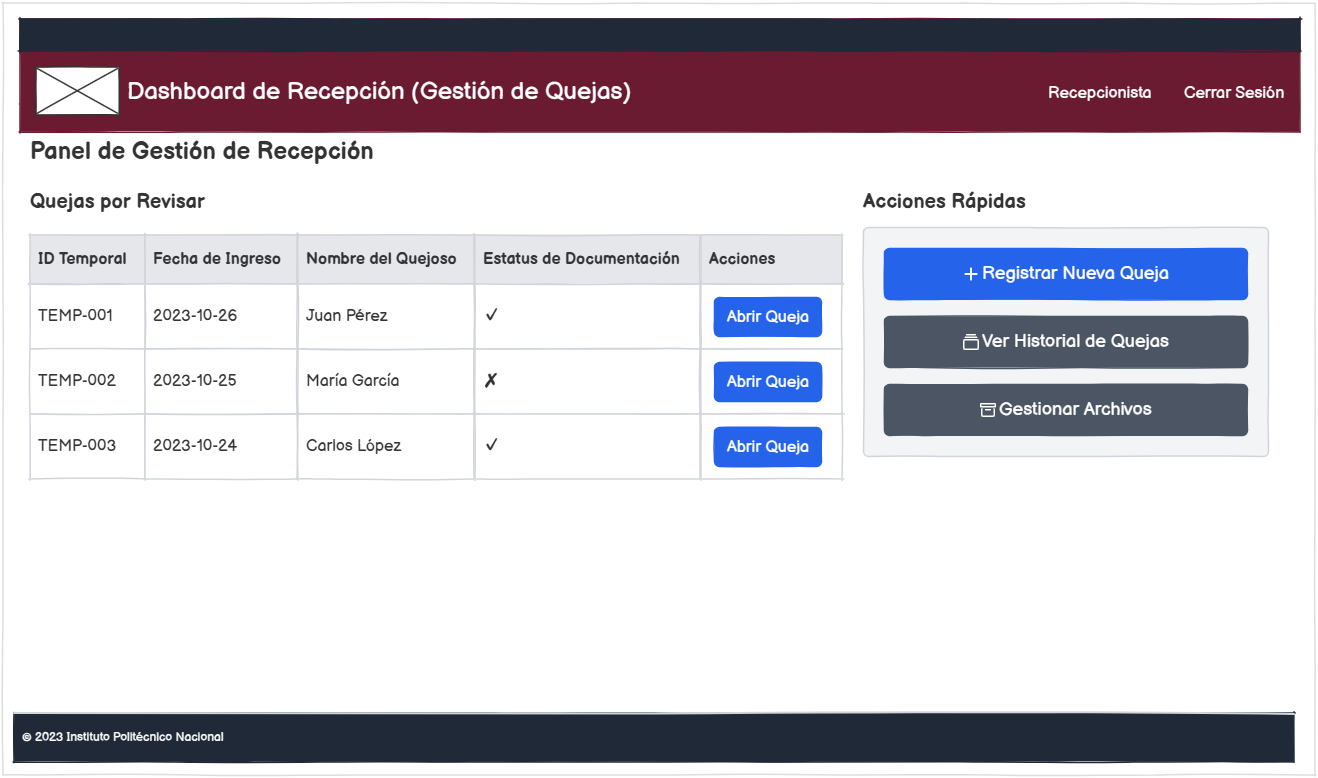
\includegraphics[width=0.65\textwidth]{imagenes/recepcion/PanelGestiónRecepción.png}
\caption{MA-04: Panel de gestión de recepción (Dashboard).}
\label{fig:ma04_dashboard_recepcion}
\end{figure}

\noindent \textbf{Descripción de la interfaz (MA-04):} \
Este tablero de control permite al personal de recepción monitorear las quejas entrantes de manera centralizada mediante una tabla operativa que utiliza identificadores temporales para registros pendientes de validación. La interfaz incluye indicadores visuales que señalan si un expediente cuenta con documentación completa, permitiendo el acceso directo al detalle de cada registro. Asimismo, un menú de acciones rápidas facilita tareas como el registro de nuevas quejas o la consulta del historial, manteniendo siempre visible el rol de recepcionista para asegurar la consistencia de los permisos.

\vspace{1cm}

% --- VISTA 05: VALIDACIÓN DE REQUISITOS ---
\begin{figure}[h]
\centering
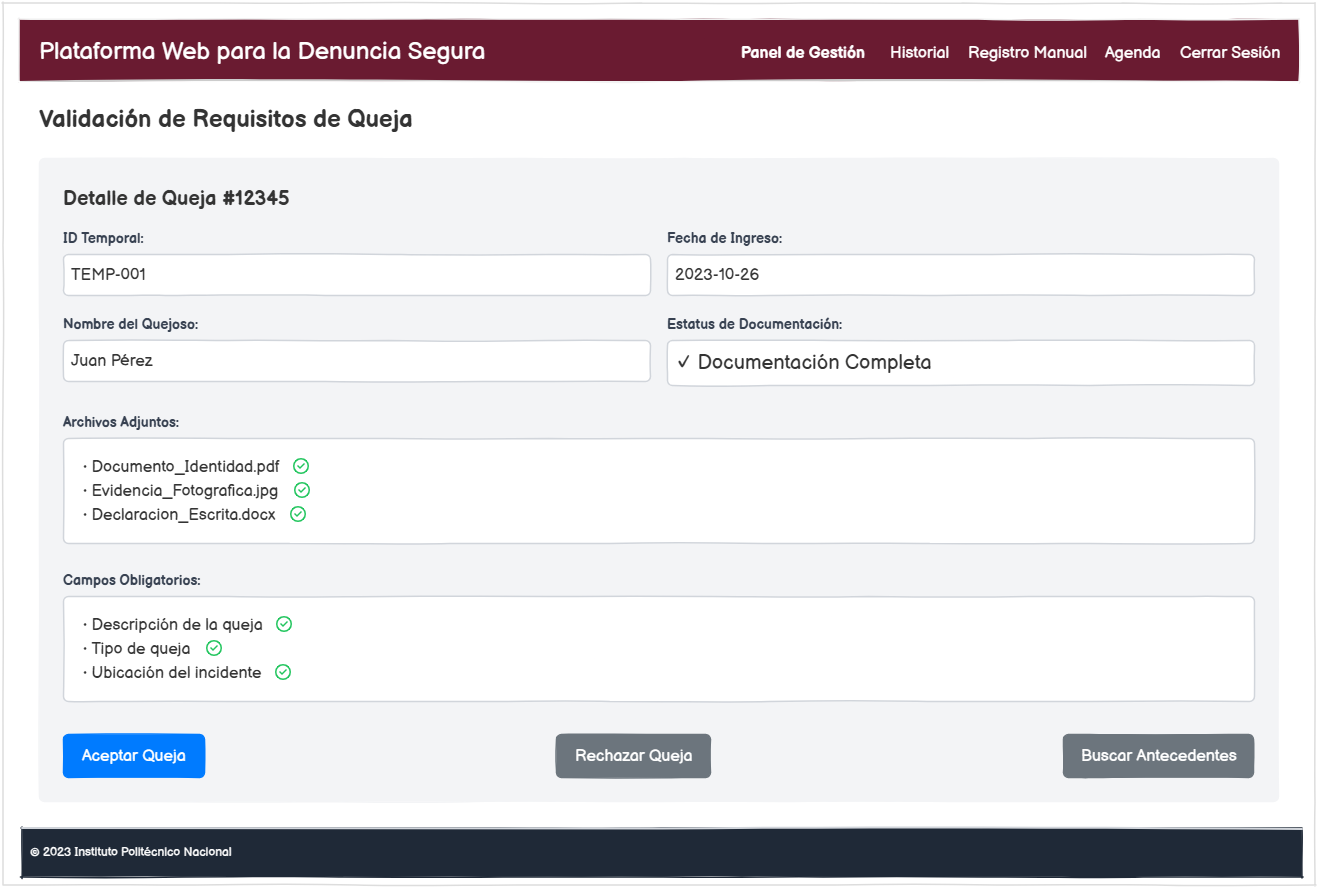
\includegraphics[width=0.65\textwidth]{imagenes/recepcion/ValidaciónRequisitosQueja.png}
\caption{MA-05: Módulo de validación de requisitos de queja.}
\label{fig:ma05_validacion_requisitos}
\end{figure}

\noindent \textbf{Descripción de la interfaz (MA-05):} \
Esta interfaz constituye el control de calidad del sistema, donde el personal asegura que cada solicitud cumpla con los estándares normativos. Presenta un resumen del expediente y un listado detallado de archivos adjuntos validados mediante iconos de verificación. El sistema obliga a la revisión de campos obligatorios como la descripción y la ubicación del incidente, concluyendo el proceso con botones de control que permiten aceptar la queja para su formalización, rechazarla por inconsistencias o realizar una búsqueda exhaustiva de antecedentes antes de su envío.

\vspace{1cm}

% --- VISTA 06: NOTIFICACIÓN DE RECHAZO ---
\begin{figure}[h]
\centering
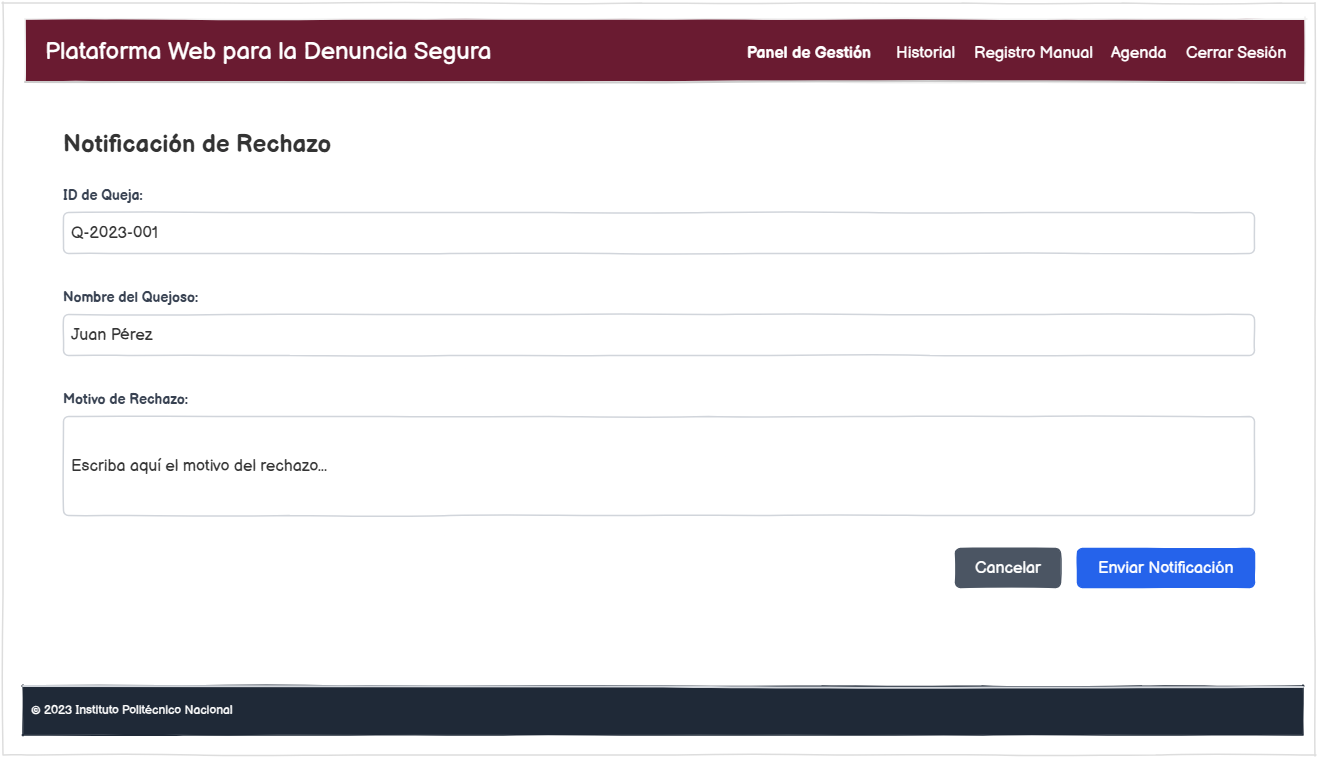
\includegraphics[width=0.65\textwidth]{imagenes/recepcion/NotificacionRechazo.png}
\caption{MA-06: Interfaz de notificación de rechazo por incumplimiento.}
\label{fig:ma06_notificacion_rechazo}
\end{figure}

\noindent \textbf{Descripción de la interfaz (MA-06):} \
Esta pantalla se activa al determinar que una solicitud no cumple con los requisitos mínimos, permitiendo informar al quejoso de manera formal sobre las deficiencias detectadas. La interfaz vincula automáticamente el ID del trámite y el nombre del usuario, ofreciendo un área de texto libre para que el administrativo redacte el motivo técnico o jurídico del rechazo. Una vez procesada la notificación, el sistema dispara un correo automático, permitiendo al personal retornar a sus labores mediante un menú de navegación persistente que conecta con la agenda e historial.

\vspace{1cm}

% --- VISTA 07: ANTECEDENTES Y CANALIZACIÓN ---
\begin{figure}[h]
\centering
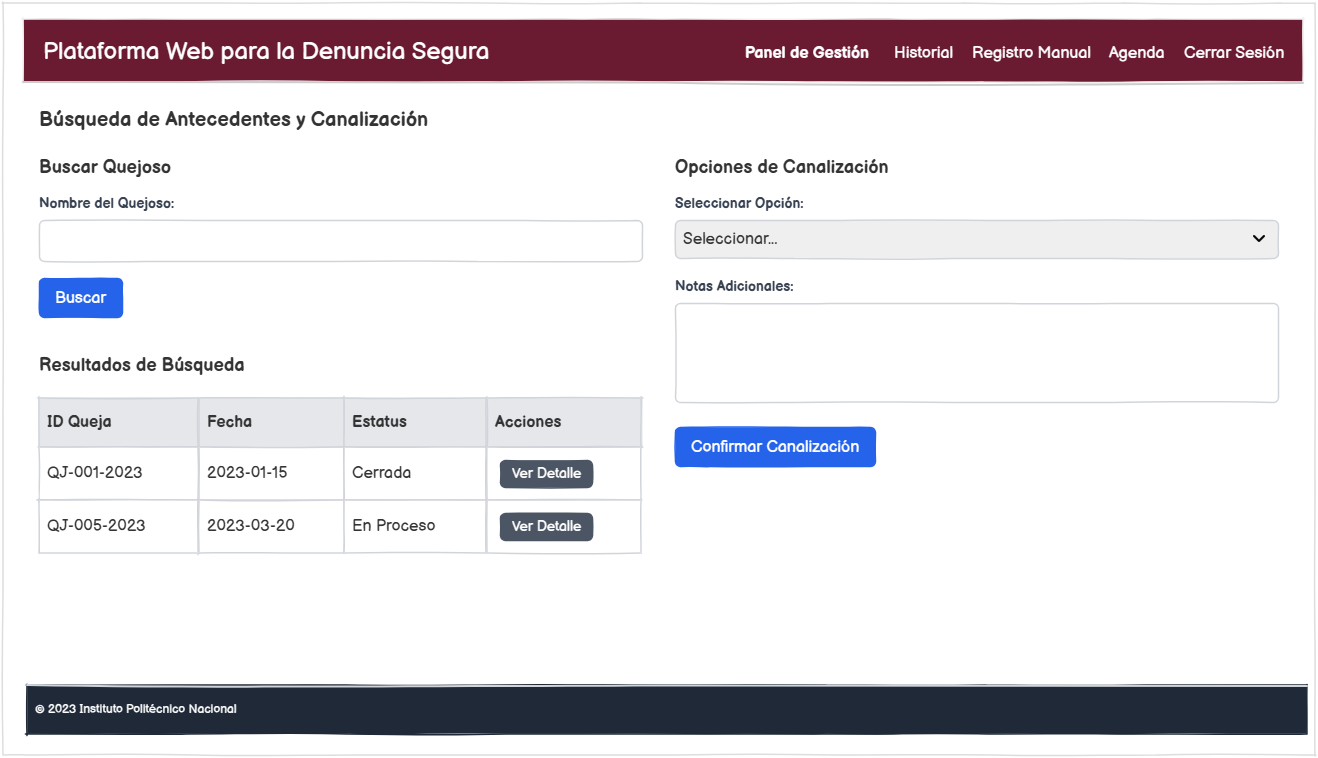
\includegraphics[width=0.65\textwidth]{imagenes/recepcion/BuesquedaAntecedentesCanalizacion.png}
\caption{MA-07: Módulo de búsqueda de antecedentes y canalización interna.}
\label{fig:ma07_canalizacion}
\end{figure}

\noindent \textbf{Descripción de la interfaz (MA-07):} \
Esta pantalla representa el último paso operativo en el área de Recepción, funcionando como motor de búsqueda y herramienta de traslado de expedientes. El sistema permite identificar procesos previos del quejoso para evitar duplicidades, mostrando una tabla de resultados con el historial de trámites anteriores. Para finalizar, el administrativo utiliza el panel de canalización para seleccionar el departamento de destino, agregando notas adicionales que orienten al siguiente analista antes de confirmar el envío y actualizar el estatus global del trámite.

\subsection{Departamento de Primer Contacto}
Este departamento se encarga de la atención personalizada al quejoso. Su función principal es realizar la entrevista inicial, analizar la naturaleza de la queja y determinar si el asunto es competencia de la Defensoría o si debe ser orientado a otra instancia.

% --- VISTA 08: BANDEJA DE ANÁLISIS ---
\begin{figure}[h]
\centering
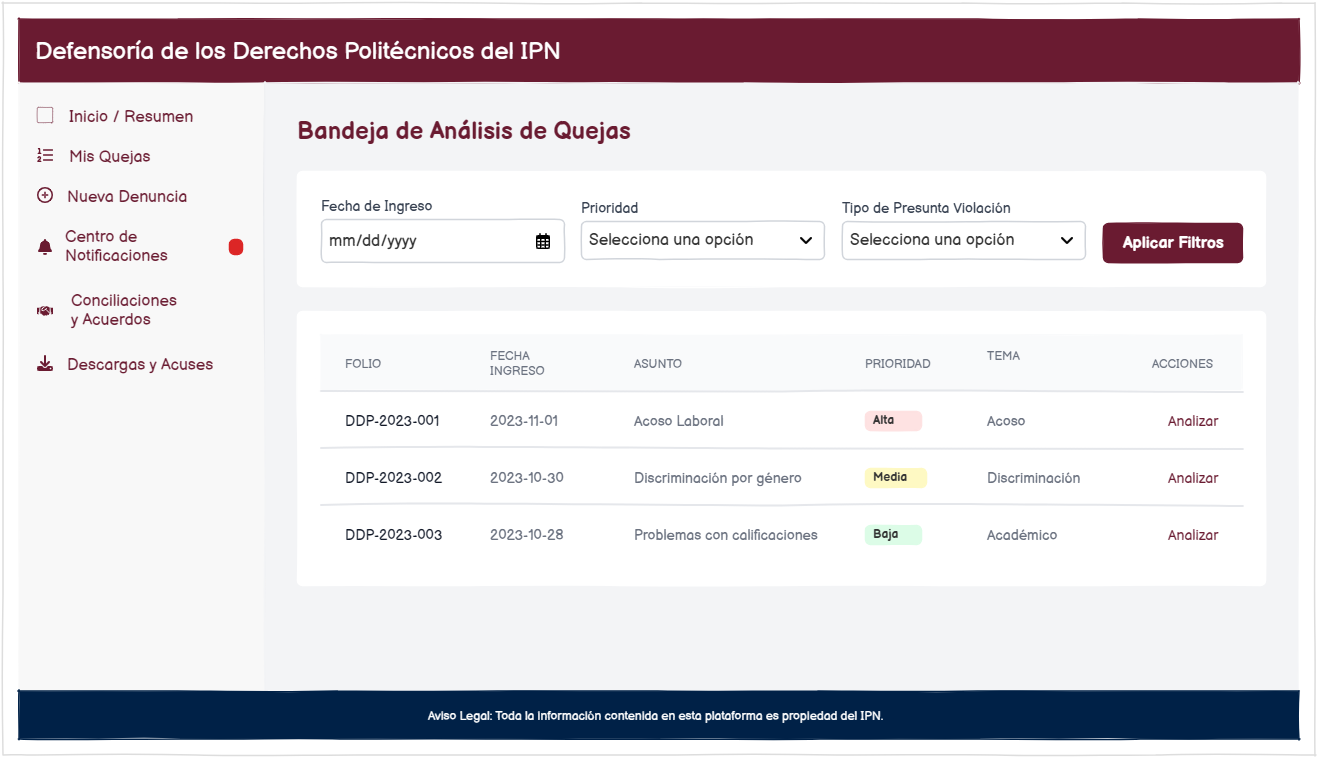
\includegraphics[width=0.65\textwidth]{imagenes/primercontacto/DashboardoAnalisisQuejas.png}
\caption{MA-08: Bandeja de análisis de quejas para Primer Contacto.}
\label{fig:ma08_analisis_dashboard}
\end{figure}

\noindent \textbf{Descripción de la interfaz (MA-08):} \
Esta interfaz constituye la herramienta principal del abogado o analista de Primer Contacto, diseñada para organizar de manera eficiente las quejas canalizadas desde el área de Recepción. La pantalla integra un módulo de filtrado avanzado que permite segmentar la carga de trabajo por fecha, prioridad y tipo de violación, facilitando la identificación de casos urgentes. A través de una tabla de gestión operativa, el personal puede visualizar los folios oficiales y los temas asignados, utilizando un sistema visual de etiquetas de colores para jerarquizar los hechos reportados. Finalmente, el control de análisis permite al funcionario acceder al detalle del expediente para iniciar formalmente la calificación jurídica.

\vspace{1cm}

\begin{figure}[h]
\centering
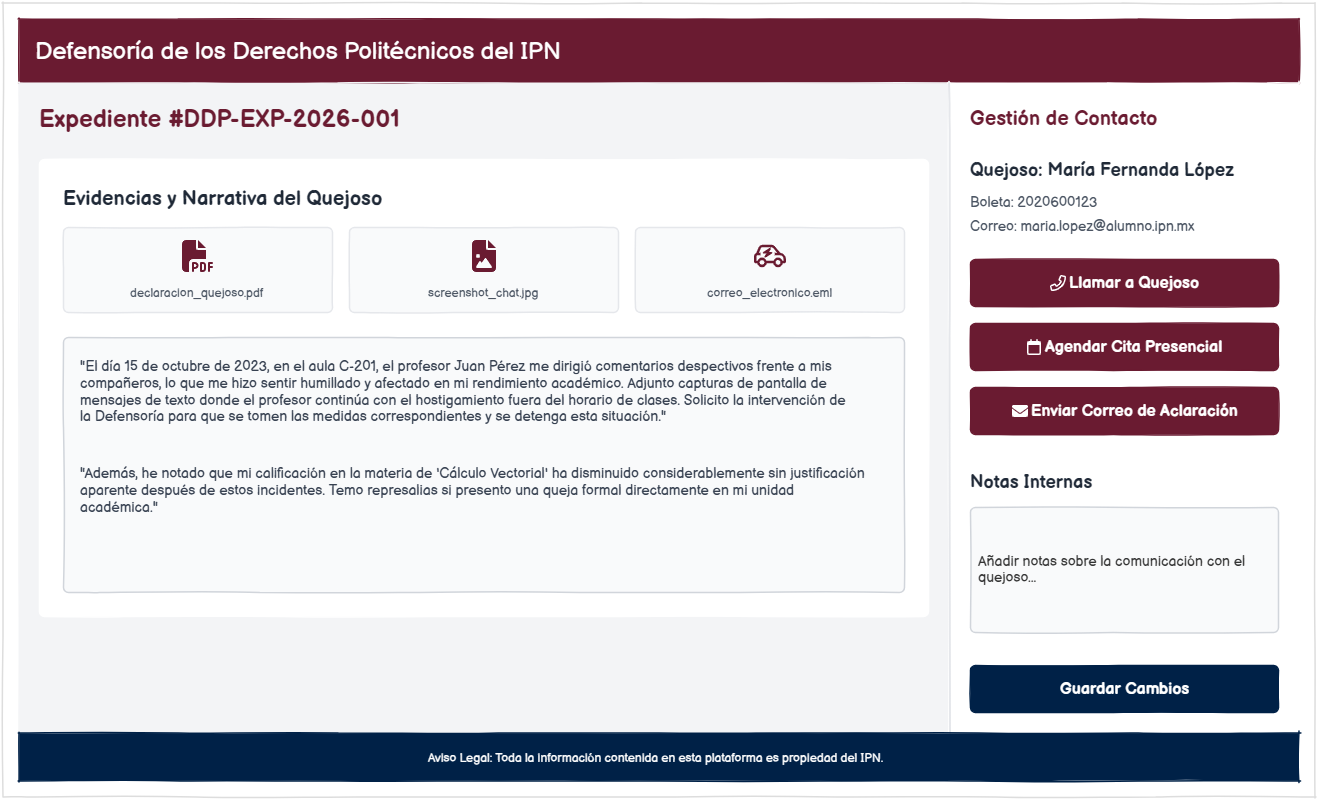
\includegraphics[width=0.65\textwidth]{imagenes/primercontacto/AnalisisExpediente.png}
\caption{MA-09: Interfaz de estudio de narrativa y evidencias.}
\label{fig:ma09_analisis_expediente}
\end{figure}

\noindent \textbf{Descripción de la interfaz (MQ-09):} \
Esta pantalla centraliza toda la información aportada por el quejoso para facilitar una evaluación legal exhaustiva por parte del analista. La interfaz dispone de un visor de evidencias con iconos diferenciados por formato, permitiendo una rápida revisión de los archivos adjuntos, junto a un área dedicada a la narrativa de los hechos para identificar presuntas violaciones de derechos. Además, se integra un panel de gestión de contacto con herramientas de comunicación inmediata para agendar citas o solicitar aclaraciones, complementado con una bitácora de notas internas donde el analista puede registrar observaciones técnicas que aseguren la continuidad del caso.

\clearpage


% --- VISTA 10: AGENDAR CITAS ---
\begin{figure}[h]
\centering
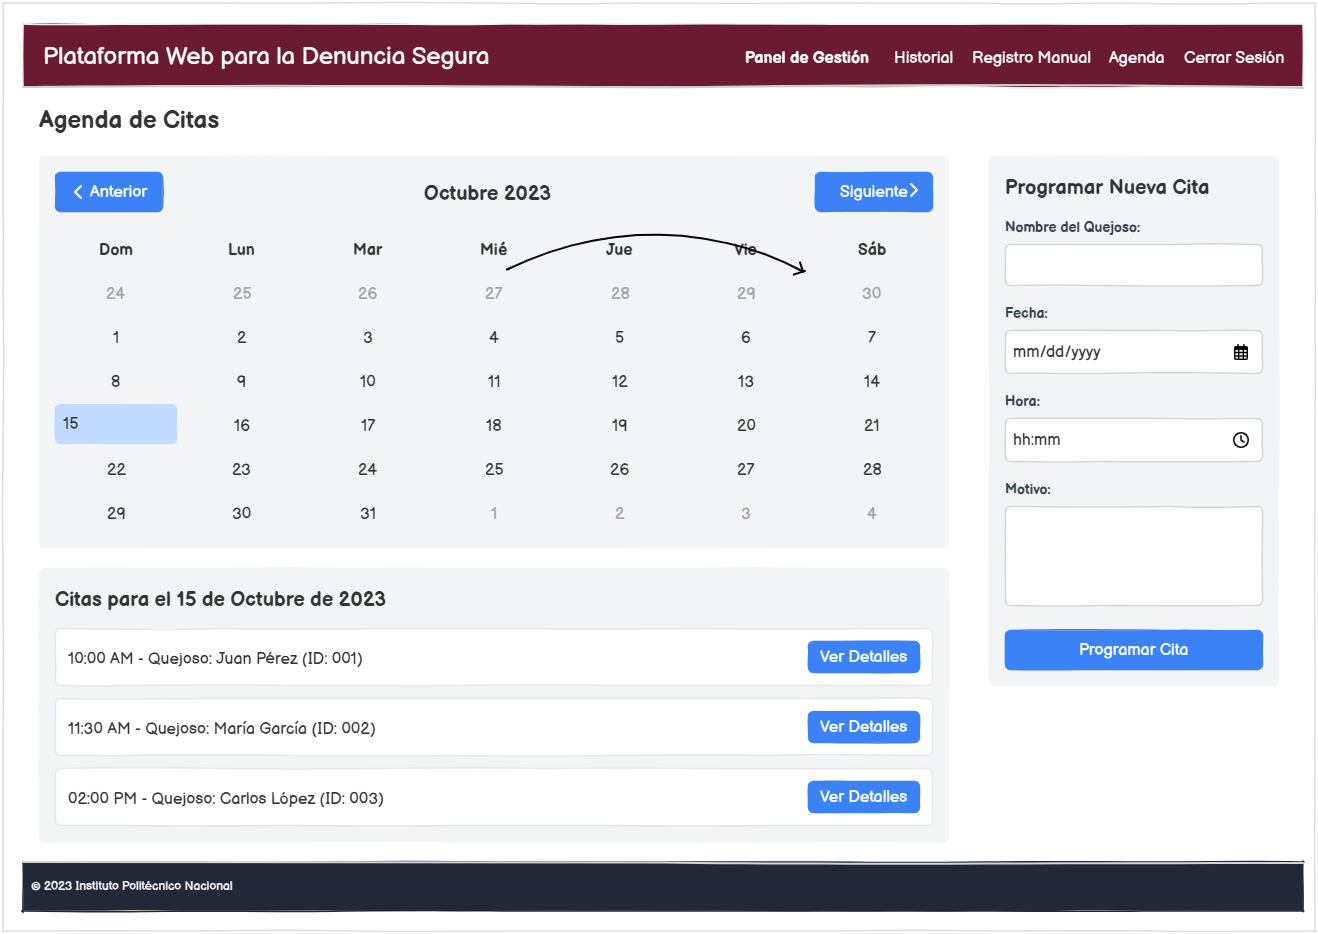
\includegraphics[width=0.65\textwidth]{imagenes/primercontacto/AgendarCitas.png}
\caption{MA-10: Módulo de agenda institucional para entrevistas de calificación.}
\label{fig:ma10_agenda_citas}
\end{figure}

\noindent \textbf{Descripción de la interfaz (MA-10):} \
Esta interfaz es fundamental para gestionar la interacción directa entre el analista y el quejoso, permitiendo organizar las diligencias necesarias para profundizar en los hechos. Presenta un calendario de disponibilidad dinámico que ayuda a evitar el traslape de horarios y optimiza el uso de las salas de entrevista, junto a un formulario lateral para capturar los detalles de cada reunión. El sistema vincula automáticamente al quejoso con una fecha y modalidad específica, manteniendo una lista de próximas entrevistas para la preparación previa del expediente. Al confirmar la cita, el estatus del trámite se actualiza automáticamente, notificando al usuario a través del portal correspondiente.

\clearpage


\begin{figure}[h]
\centering
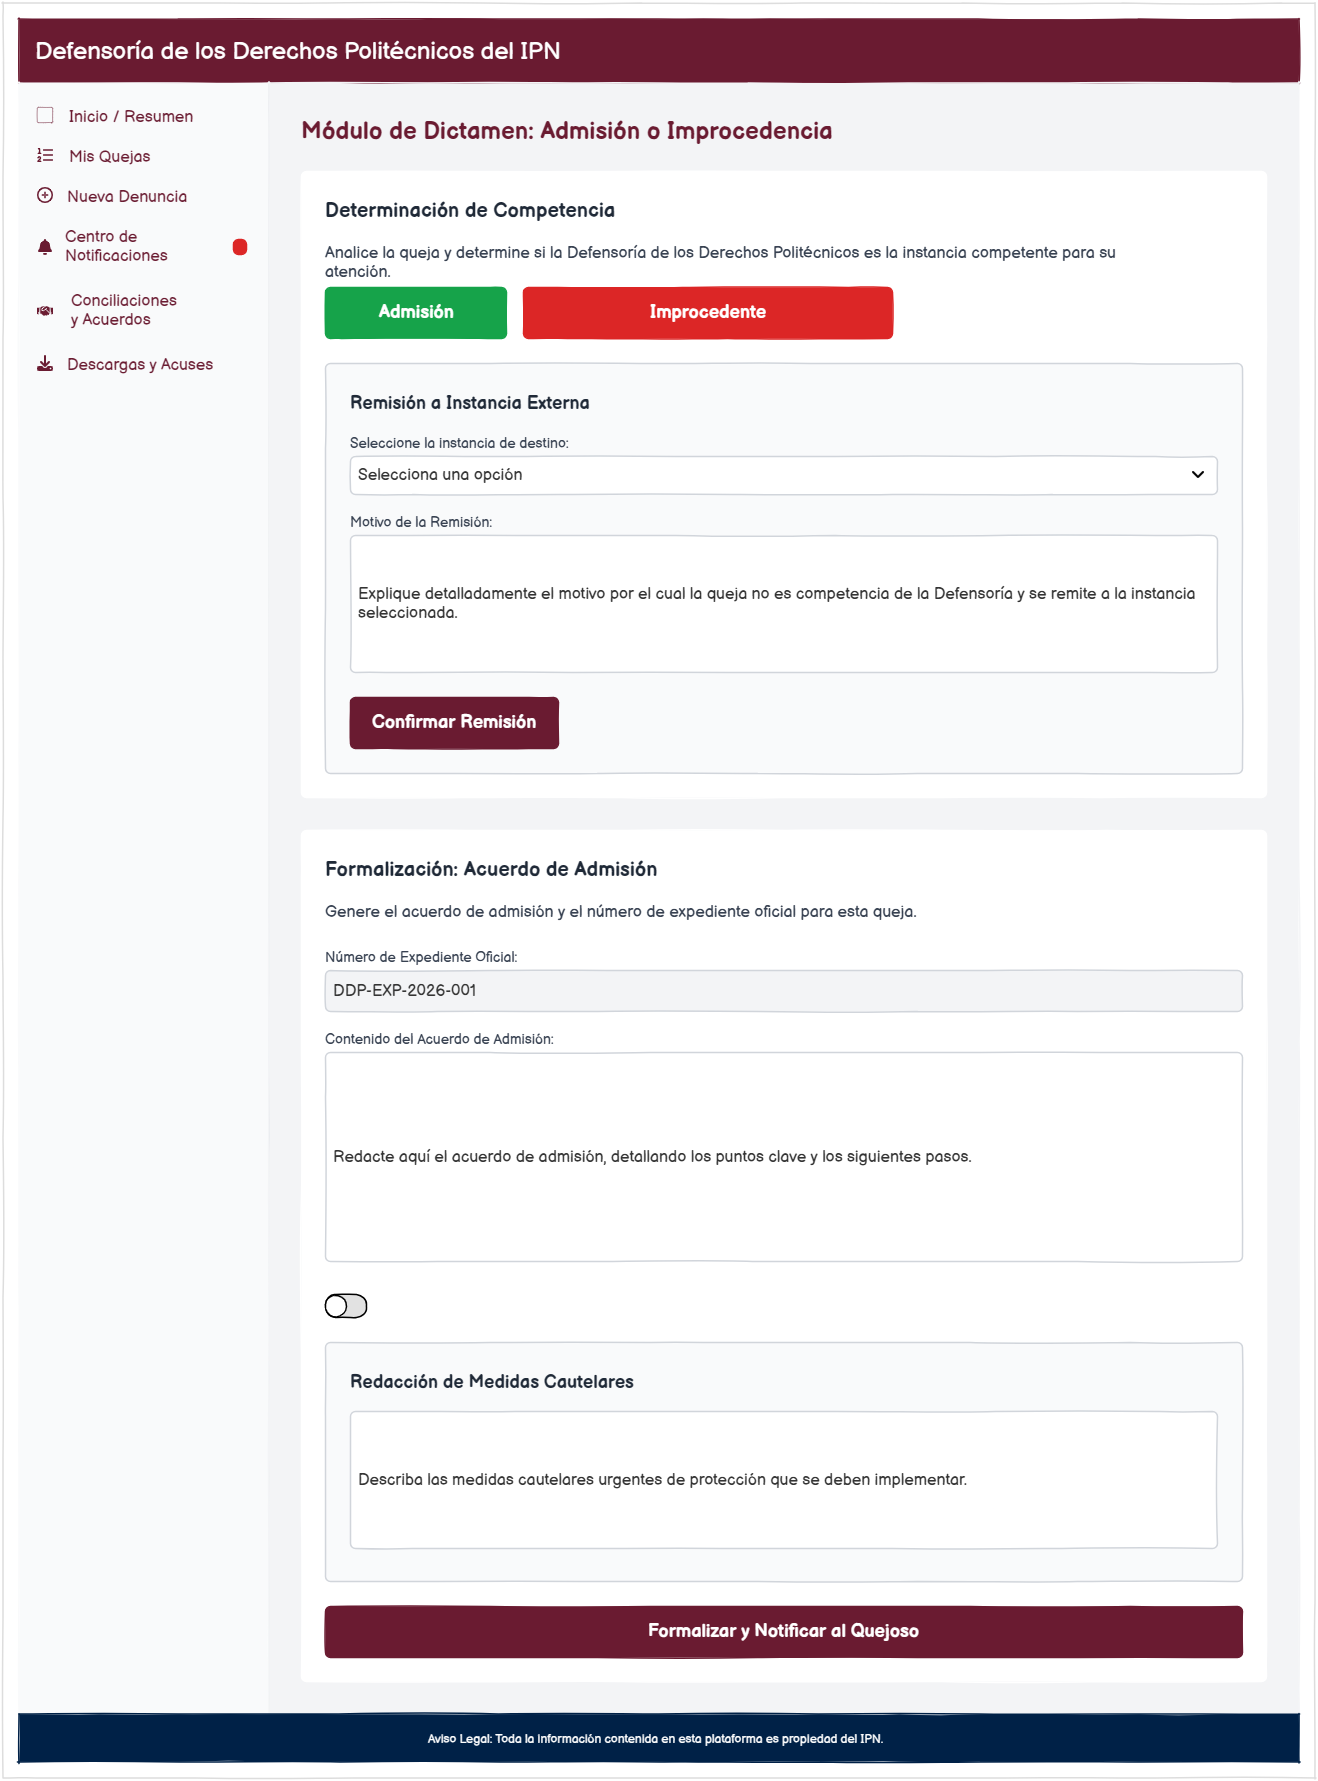
\includegraphics[width=0.65\textwidth]{imagenes/primercontacto/DictamenCompetencia}
\caption{MA-11: Módulo de dictamen de admisión o improcedencia.}
\label{fig:ma11_dictamen_competencia}
\end{figure}

\noindent \textbf{Descripción de la interfaz (MA-11):} \
Esta es la pantalla de resolución técnica donde se decide formalmente el curso legal de la queja presentada. El sistema ofrece botones de selección de alto contraste para definir la procedencia del caso, habilitando secciones específicas según la decisión tomada, ya sea para redactar los motivos legales de una improcedencia y su remisión externa, o para generar el número de expediente oficial en caso de admisión. La interfaz incluye también un control para la redacción de medidas cautelares urgentes en situaciones que requieran protección inmediata del quejoso. Una vez procesado el dictamen, el sistema formaliza el acto jurídico y prepara la notificación automática para el usuario.


\clearpage

% --- VISTA 12: FINALIZACIÓN Y NOTIFICACIÓN ---
\begin{figure}[h]
\centering
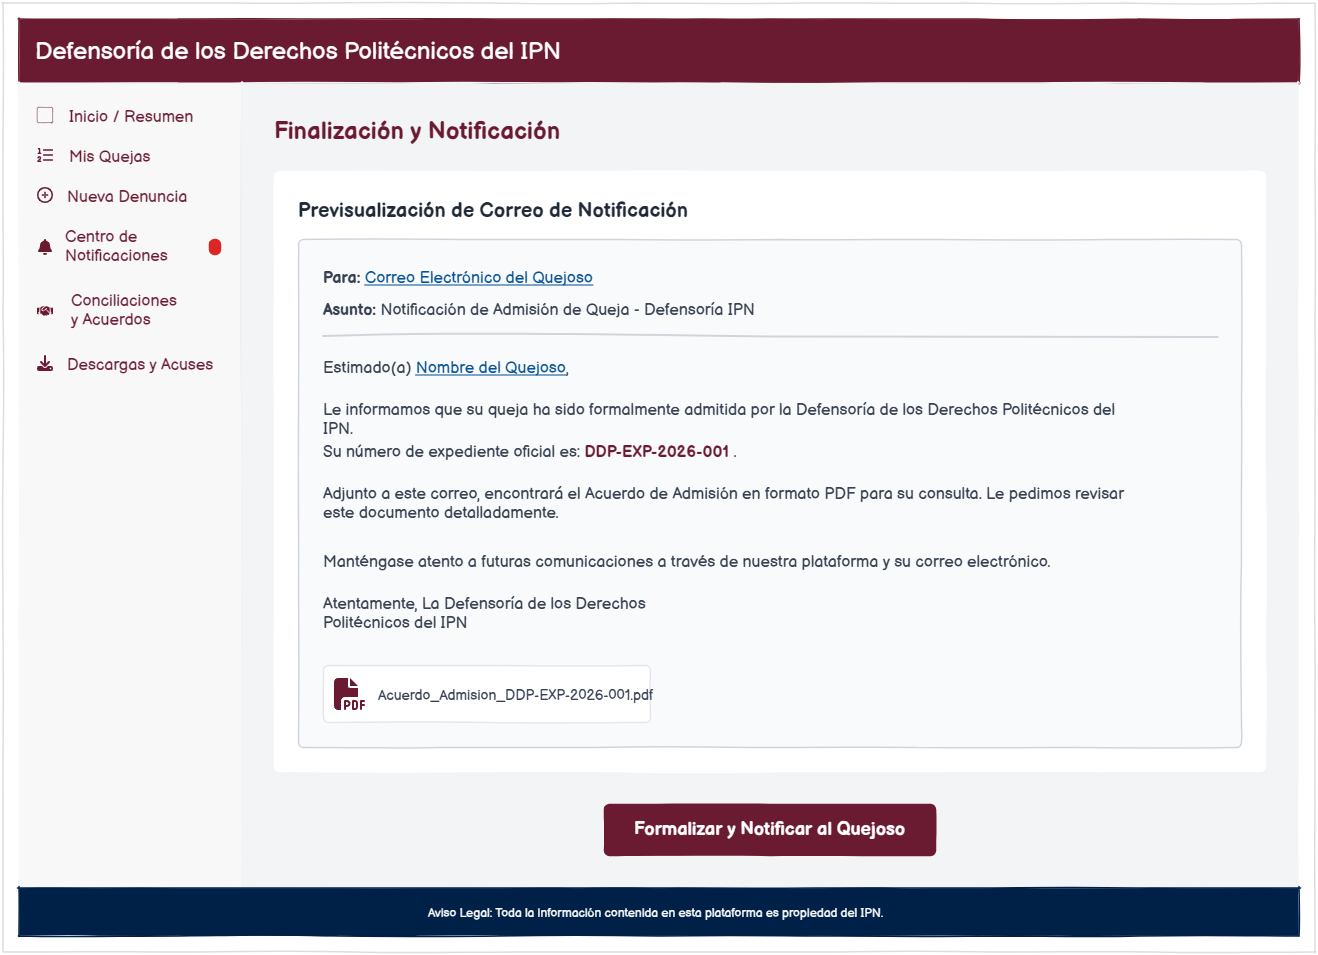
\includegraphics[width=0.65\textwidth]{imagenes/primercontacto/FormalizacionNotificacion.png}
\caption{MA-12: Interfaz de previsualización y notificación de admisión oficial.}
\label{fig:ma12_finalizacion_notificacion}
\end{figure}

\noindent \textbf{Descripción de la interfaz (MA-12):} \
Esta pantalla constituye el paso final del departamento de Primer Contacto antes de trasladar el expediente al área de instrucción en la Subdefensoría. Su propósito principal es garantizar la transparencia mediante una previsualización de la notificación oficial, permitiendo al analista verificar el cuerpo del correo electrónico y el número de expediente asignado. La interfaz muestra el archivo PDF del acuerdo de admisión vinculado y ofrece un botón de formalización que ejecuta simultáneamente el envío de la notificación y el cambio de estatus a "Admitida". De esta manera, se habilita el acceso al expediente para el siguiente departamento mientras el personal administrativo mantiene visibilidad sobre otras tareas pendientes en el entorno de gestión.

\end{appendices}